\chapter{Proof Extraction}
\label{chapter:chapter_3}

\chapabstract{\textit{A program that only lives on paper is not a program.}}

With our theorycrafting over, we have in our hands an uninstantiated descriptive model of syntactic and semantic composition, promising to capture dependency relations while keeping both its feet set firmly in type theory.
Unfortunately, it is well attested by now that ``all models are wrong...''~\cite{doi:10.1080/01621459.1976.10480949}.
Any promise of theoretical universality, cognitive plausibility, linguistic intrinsicness or what have you, would require some degree of handwaving and conjencturing that I am not comfortable with.
What is undisputable, however, is the nobility of our goals and the purity of our tools: the \textit{omniversality} of the $\lambda$ calculus~\cite{wadler2015propositions} asserts that our modeling approach is not some ad hoc machinery designed to tackle a highly localized problem, but the one and only programming language ever worth writing. 
Beyond purpose and methodology, and having \textit{a priori} given up any ideation of truth, the only measure of success for our model is that of its utility (``...but some are useful'', ~\cite{doi:10.1080/01621459.1976.10480949}).
This sets up a new research imperative: we must prove the model useful!

``Oof, that's a tricky one'', you might say, and you wouldn't be wrong.
Thankfully, there are two tried and tested ways to proceed.
The first is the way of the scholar, which requires a rare combination of high intellectual capacity, strong persuasive skills and a pinch of luck.
It starts off with some profound abstract thinking, gradually overtaken by agressive campaigning: bashing the competition at workshops and conferences, making bold claims and generating traction at any chance given (optionally over social media platforms, for the modernists), eventually building a cult of personality, and finally resting on your laurels as the hype becomes self-sustainining; at long last, utility affirmed by popular approval.
This path, sometimes called the scientific method, is a rather involved and painstakingly slow process, a high stakes gamble that only starts yielding profits in the long run; as such, it greatly benefits from the nourishment of a stable work environment.
More befitting the modern paradigm of the mobile, adaptive, multi-purpose researcher is the alternative path, the way of the engineer.
A shorter term investment, it requires only the acquirable skills of endurance and hardheadedness, and offers a recipe that's easier to follow: simply swing at it until it cracks.
After a lot of obsessive iteration and self-correction (interchanged with the occasional feeling of despair), (f)utility will sooner or later be affirmed by cold, hard numbers.
We'll go for this one.

This choice has some methodological repercussions.
Under more tranquil circumstances, we'd wait for the theory to be disseminated, criticized, adapted, error-corrected and returned to sender, before finally moving on; it being a theory of language, this would entail a thorough qualitative analysis of several kinds of linguistic phenomena, coupled with a theoretical investigation of what it can or cannot adequately capture.
We are however in a compressed timeframe, forcing our hand into putting it straight to the test; the pragmatic approach is then to try and directly align it with real-world linguistic data at scale, and hope for the best.
The process, called \textit{proof extraction}, revolves around ``proving''  some source corpus of syntactically annotated sentences via the design and application of an algorithm tasked with translating the existing annotation format into derivations of the target grammar -- in our case, a grammar of dependency-enhanced compositional assembly.
Proof extraction serves a ternary purpose.
One, it gives us access to an uncompromisingly realistic testbed upon which we can immediately inspect and iteratively finetune the specifics of the grammar logic.
Two, it fills in for a strict and impartial external critic in providing a quantitative evaluation regime -- at each point in time, we are able to measure the proportion of source analyses (and corresponding linguistic phenomena) the algorithm provides a (reasonable) output for.
And three, the end-yield of this process has merit of its own.
As a derived dataset, it is first a building block necessary for populating the computational toolshed of the theory, and also a public resource for the world to with as they please.

Before we get started, let me apologize for the gloomy mood that might permeate this chapter here and there.
Proof extraction has been the most gruesome and iterated aspect of my path to doctorhood, its maintance and upkeep having an almost annual recurrence (with nothing festive about it).
For the sake of scientific transparency, I have no choice other than to expose it in all its horrific details, but it might be that my fatigue of the topic occassionally reflects in a less-than-usually interesting prose.

\section{Preliminaries}
\subsection{The Dutch Language}
For our linguistic inquiries, the focus will be on Dutch.
Other than being the language I was contractually obliged to conduct this research on, Dutch is an interesting specimen, the idiosyncracies of which have in the past proven quite a topic of debate for others, and a source of headaches for myself.
I don't have any intention (or delusion of competence) to casually throw a detailed exposition of the Dutch grammar here, but a brief and superficial typological overview might help smooth the transition into the what is to come.
If the section has the opposite effect to the one intended, know that I'll hold no grudge if you skip ahead.

But first things first.
Dutch is a West Germanic language, spoken primarily in the Low Countries within Europe by some 25 million speakers.
Owing to the Netherlands' nasty colonial history, Dutch has left a noticeable mark on the global linguistic atlas: it has played a primary role in the evolution of Afrikaans and, to a far lesser extent, Indonesian, while native Dutch speakers can be found as far as South America and the Dutch Carribean region.
Demographics aside, the language is said to be one of the closest relatives of English and German, sharing many of their morphosyntactic characteristics -- we'll go through some of those together.
The abbrevations in the glosses to follow are industry standard, you can find their transcriptions in Table~\ref{table:gloss_abbreviations} of Appendix~\ref{sec:abbrevations}.
Any internal inconsistencies are deliberate: I am trying to gloss only those features relevant to the local discussion.

\subsubsection{The Noun Phrase}
\paragraph{Nouns}
Dutch nouns have three grammatical genders: the masculine, the feminine and the neuter.
The masculine and feminine genders are morphologically indistinguishable -- telling them apart is done on the basis of the lexicon alone.
\begin{exe}
\ex\label{gloss:genders}
\begin{xlist}
\ex
\gll \textit{de} \textit{aard}\\
the earth(\abbrv{m})\\
\ex
\gll \textit{de} \textit{zee}\\
the sea(\abbrv{f})\\
\ex
\gll \textit{het} \textit{bos}\\
the forest(\abbrv{n})\\
\end{xlist}
\end{exe}
There's two numbers, the singular and the plural, the latter constructed with the aid of the suffix \textex{-en} or rarely \textex{-s}, depending on the noun.
\begin{exe}
\ex 
\begin{xlist}
\ex
\gll \textit{de} \textit{zeven} \textit{zee-\"{e}n}\\
the seven sea-\abbrv{pl}\\
\glt{`the seven seas'}
\ex
\gll \textit{de} \textit{trekvogel-s}\\
the  migratory.bird-\abbrv{pl}\\
\glt{`the migratory birds'}
\end{xlist}
\end{exe}
Case markings are not overtly realized, except for some mostly frozen leftovers from the distant past -- their functionality has largely been replaced by word order constraints, with the indirect object (formerly in the dative) preceding the direct object (formerly in the accusative), and periphrastic constructions, with the preposition \texttr{aan}{to} used to indicate indirect objects (see Gloss~\ref{gloss:ido} later on), and \texttr{van}{of} to substitute the genitive.
\begin{exe}
\ex
\gll \textit{het} \textit{oog} \textit{van} \textit{de} \textit{geest}\\
the eye of the mind\\
\glt{`the mind's eye'}
\end{exe}
A cute peculiarity of Dutch is the strikingly common use of a productive diminutive form, denoting either small size or an affectionate disposition -- diminutives are formed with the suffix \textex{-tje} or regionally \textex{-ke}, and are always neuter (notice the gender change of Gloss~\ref{gloss:gender_change}).

\paragraph{Determiners}
Determiners precede the noun and match its gender and number.
There are two articles: the definite, and the indefinite.
The definite has two singular forms \textex{de}/\textex{het} (non-neuter/neuter) and a single plural \textex{de}. 
Non-neuter forms are used for both masculine and feminine (refer back to Gloss~\ref{gloss:genders}).
\begin{exe}
\ex\label{gloss:gender_change}
\begin{xlist}
\ex
\gll de klein-e vogel\\
the(\abbrv{nn.sg}) small-\abbrv{def} bird\\
\glt{`the small bird'}
\ex
\gll het klein-e vogel-tje\\
the(\abbrv{n.sg}) small-\abbrv{def} bird-\abbrv{dim}\\
\glt{`the small birdie'}
\end{xlist}
\end{exe}
The indefinite \textex{een} is gender-agnostic, and has no plural form.
\begin{exe}
\ex
\begin{xlist}
\ex\label{gloss:indef_adj_sg_n}
\gll een donker lied\\
a dark song\\
\glt{`a dark song'}
\ex 
\gll donker-e lied-eren\\
dark-\abbrv{pl} song-\abbrv{pl}\\
\glt{`dark songs'}
\end{xlist}
\end{exe}
Indefinite pronouns can be used to convey universal or existential quantification and negation, materializing as substitutes for determiners (e.g. \texttr{alles}{all}, \texttr{sommige}{some}, \texttr{geen}{no}, etc.), or as stand-alones (e.g. \texttr{iets}{something}, \texttr{niets}{nothing}, etc.).
\begin{exe}
\ex
\gll Alle mensen willen iets, sommige willen alles.\\
all people want something some want everything\\
\glt{`All people want something, some want everything.'}
\end{exe}
Possessive and demonstrative pronouns can also enact determiners, both uninflected (except for the first person plural \textex{ons} which inflects like an indefinite adjective, see next paragraph).
\begin{exe}
\ex
\gll De eend is mijn favoriet vogel.\\
the duck is my favorite bird\\
\glt{`The duck is my favorite bird.'}
\ex\label{gloss:ido}
\gll Het bos is onz-e tempel.\\
the forest is our-\abbrv{def} temple\\
\glt{`The forest is our temple.'}
\end{exe}
There's two types of demonstrative pronouns: the proximal \textex{deze/dit} (plural \textex{deze}) and the distal \textex{die/dat} (plural \textex{die}).
The last two do double duty as relative pronouns -- more on that later.
When used to substitute (rather than determine) a noun in a copula, each variant reverts to its neuter singular form.
\begin{exe}
\ex
\begin{xlist}
\ex
\gll Deze bergen zijn hoog.\\
these(\abbrv{pl}) mountains are tall\\
\glt{`These mountains are tall.'}
\ex
\gll Dit zijn mijn bergen.\\
this(\abbrv{n}) are my mountains\\
\glt{'These are my mountains.'}
\end{xlist}
\end{exe}

\paragraph{Adjectives}
Adjectives used as nominal modifiers find their place between the determiner and the head noun.
They appear inflected with an \textex{-e} affix in all cases except for the idefinite use with a neuter singular noun (refer back to Gloss~\ref{gloss:indef_adj_sg_n}, contrast with \ref{gloss:gender_change}).
The same affix applies to nominalized adjectives, which can allow the ommission of a contextually implied noun, or be used independently as an abstract concept or a quantifying property.
\begin{exe}
\ex
\gll dood aan het heilig-e\\
death to the holy-\abbrv{nmlz}\\
\glt{`death to the holy'}
\ex
\gll De zachtmoedig-en zullen niets be\"{e}rven.\\
the meek-\abbrv{nmlz.pl} shall nothing inherit(\abbrv{inf})\\
\glt{`The meek shall inherit nothing.'}
\end{exe}
An alternative inflection with a \textex{-s} affix marks the partitive use, when the adjective modifies an indefinite pronoun.
\begin{exe}
\ex
\gll iets ernstigs-s\\
something grave-\abbrv{ptv}\\
\glt{`something grave'}
\end{exe}
The language provides acccess to a comparative and a superlative form, via the affixes \textex{-er} and \textex{-ste} respectively, or periphrastically with \texttr{meer}{more} and \texttr{meest}{most}.
\begin{exe}
\ex
\gll \textit{het} \textit{donker-ste} \textit{lied}\\
the(\abbrv{n.sg}) dark-\abbrv{sup} song\\
\glt{`the darkest song'}
\end{exe}

\paragraph{Personal Pronouns}
Noun phrases can be substituted by personal pronouns, which in Dutch are morphologically marked for case and gender.
The nominative is used for the subject position, the genitive corresponds to the possessive determiners discussed earlier, and the accussative is used to denote objects.
\begin{exe}
\ex
\gll Ik zie een vreemde man in de spiegel.\\
I(\abbrv{nom}) see a strange man in the mirror\\
\glt{`I see a strange man in the mirror.'}
\ex
\gll Hij merkt mij op.\\
he(\abbrv{nom}) perceives me(\abbrv{acc}) on\\
\glt{`He notices me.'}
\end{exe}
A dative form is sometimes exceptionally used for indirect objects in the third person plural.
Depending on the regional variation, personal pronouns must match the grammatical gender of the noun they refer to, or simply default to the neuter (reserving the masculine and feminine forms for animates).
Third person singulars are also interchangeable with the appropriate demonstratives.
Personal pronouns come in two variants: the stressed (emphatic) and the unstressed (standard).

\subsubsection{The Verb}
\paragraph{Conjugation}
In their citation form, verbs match their infinitival versions, regularly consisting of the verbal stem plus \textex{-en}.
Verbal conjugation patterns distinguish between two grammatical tenses, the non-past and the past, and three moods, the indicative, the subjunctive and the imperative, of which the first two are morpohologically conflated.
Each pattern is parameterized by person and number.
Aspectual flavours, passivization and an explicit future are accessible as productive constructions with modals, the latter being the common culprits of irregular conjugation.

\paragraph{Participles}
Participles exist for both tenses, and have a multitude of uses.
The present participle is formed by affixing \textex{-de}, and is commonly employed as an duration-denoting adjective or adverb, always inflected in the first case, and optionally in the second.
\begin{exe}
\ex
\gll de zweven-de vrouw\\
the levitate-\abbrv{prs.ptcp} woman\\
\glt{`the levitating woman'}
\end{exe}
Rarely, it can be used as a complement to the auxiliary \texttr{zijn}{to be} to produce a kind of present continuous.
Present participles of transitives can attach to the end of their object nouns, appearing as fused compounds.
The past participle is more versatile.
Regular past participles are formed by prefixing \textex{ge-} to the verbal stem (morphophonological terms and conditions may apply) and substituting the infinitival suffix for either \textex{-t}, \textex{-d} or nothing, depending on the stem's last phoneme.
Like the present participle, it can be used as an adjective, denoting now a completed event.
\begin{exe}
\ex
\gll beelden met ge-sloten ogen\\
images with \abbrv{pst.ptcp}-close eyes\\
\glt{`closed eye visuals'}
\end{exe}
Combined with with the modal \texttr{hebben}{to have} (or exceptionally \textex{zijn} for unaccusatives and verbs of movement), it produces the perfect tense.
\begin{exe}
\ex
\end{exe}
Combined with the modals \texttr{worden}{to become} and \texttr{zijn}{to be}, it produces the passive voice and its perfect tense.

\paragraph{Infinitives}
Infinitival forms commonly occur as the verbal complements of a modal, auxiliary or perception verb.
\begin{exe}
\ex
\gll Ik wil slapen.\\
I want sleep(\abbrv{inf})\\
\glt{`I want to sleep.'}
\end{exe}
Depending on the modal, the preposition \texttr{te}{to}, or the discontinuous \texttr{om ... te}{to}, may be either necessary, optionally admissible or completely disallowed -- if one does manifest, it precedes the infinitive.
\begin{exe}
\ex
\gll Ik probeer te schrijven.\\
I try to write(\abbrv{inf})\\
\glt{`I try to write.'}
\end{exe}
The discontinuous variant is only selected for by specific verbs -- it can enclose linguistic material, like the infinitive's object or any adverbs modifying it.
\begin{exe}
\ex
\gll Ik dwing mezelf om wat te schrijven.\\
I force myself \_ something to write(\abbrv{inf})\\
\glt{`I force myself to write something.'}
\end{exe}
An infinitive directly following \textex{aan het} can combine with \textex{zijn} to construct the continuous aspect, in either the present or the past tense.
\begin{exe}
\ex
\gll Ik ben aan het schrijven.\\
I am in the write(\abbrv{inf})\\
\glt{`I am writing.'}
\end{exe}
Infinitives are also often nominalized, the resulting nominals being singular neuters.
\begin{exe}
\ex
\gll Het schrijven is pijnlijk.\\
The write(\abbrv{inf}) is painful\\
\glt{`The writing is painful.'}
\end{exe}

\paragraph{Separable Verbs} 
The verbal lexicon contains several compound items comprised of a preposition and a verbal stem, usually with a compositional meaning.
The stem is separated from its prepositional prefix when the verb heads a matrix clause, in which case the preposition is moved to the end of the clause -- in all other cases, including the finite form in subordinate clauses, the two remain attached.
When inflecting for the perfect, the prefix applies to the stem (i.e. after the preposition).

\subsubsection{The Sentence}
By far the most fun aspect of Dutch is its absolutely wild sentential word order.

\paragraph{Main Clauses}
The main clauses inspected so far emanate a false sense of safety, coming off as SVO at first glance, with participles used for the passive voice and the perfect tense pushed to the right edge of the clause.
The truth is far more sinister -- the verb is placed there only by exception, abiding by the V2 rule that has it appear second for matrix clauses only.
The effect becomes apparent when employing a preverbal adverb -- in Gloss~\ref{gloss:simple_smain_v2}, both the subject and its predicate complement follow the verb in a VSO pattern.


\paragraph{Questions and Imperatives}
When it comes to questions, things look familiar again.
Line in English, wh-questions begin with an interrogative pronoun or adverb (e.g. \texttr{wie}{who}, \texttr{wat}{what}, \texttr{welk}{which}, \texttr{waarom}{why} etc.), which is immediately followed by the conjugated verb (Gloss~\ref{gloss:simple_whq}).
In direct questions without an interrogative, as well as positive imperatives, the verb is placed first (Glosses~\ref{gloss:simple_sv1_q} and \ref{gloss:simple_sv1_imp}).
In negative imperative sentences and impersonal commands, the infinitival is placed last.

\begin{exe}
\ex
\begin{xlist}
\ex\label{gloss:simple_smain}
\gll Frans verkoop-t kaas.\\
Frans sell-\abbrv{prs.3sg} cheese\\
\glt{`Frans sells cheese.'}
\ex\label{gloss:simple_smain_v2}
\gll Morgen verkoop-t Frans kaas.\\
tomorrow sell-\abbrv{prs.3sg} Frans cheese\\
\glt{`Frans will sell cheese tomorrow.'}
\ex\label{gloss:simple_sv1_q}
\gll Verkoop-t Frans kaas?\\
sell-\abbrv{prs.3sg} Frans cheese\\
\glt{`Does Frans sell cheese?'}
\ex\label{gloss:simple_whq}
\gll Wie verkoop-t kaas?\\
who sell-\abbrv{prs.3sg} cheese\\
\glt{`Who sells cheese?'}
\ex\label{gloss:simple_sv1_imp}
\gll Verkoop kaas!\\
sell(\abbrv{imp}) cheese\\
\glt{`Sell cheese!'}
\end{xlist}
\end{exe}

\paragraph{Subordinate Clauses}
Subordinate clauses is where things really get interesting.
Unaffected by the V2 rule, the word order turns out to be SOV; this affects indirect questions, verbal complements and relative clauses alike.
Indirect questions are straightforward -- modulo the word order permutation, they match their direct counterparts.
\begin{exe}
\ex\label{gloss:embedded_q}
\gll Weet je wie kaas verkoopt?\\
know you who cheese sells\\
\glt{`Do you know who sells cheese?'}
\end{exe}
Infinitives in non-nested verbal complements are likewise just pushed to the end of their clause.
\begin{exe}
\ex\label{gloss:simple_vc}
\gll Frans wil koopman worden.\\
Frans wants merchant be(\abbrv{inf})\\
\glt{`Frans wants to be a merchant.'}
\end{exe}
Relative clauses are instigated by relative adverbs and pronouns.
Interestingly, the language does not make an overt distinction between an object- and a subject- relative pronoun; combined with the SOV word order, and the absence of case markings, the effect is that the two relative clause types end up having the exact same surface form when the grammatical gender of the antecedent noun and the non-gap embedded argument are the same -- contrast the two sentences below.
\begin{exe}
\ex\label{gloss:rc_ambiguity}
\begin{xlist}
\ex
\gll het geheim dat een bos verbergt\\
the secret(\abbrv{n}) that a forest(\abbrv{n}) hides\\
\glt{
\begin{enumerate}[topsep=0pt]
	\item `the secret the hides a forest'
	\item `the secret that a forest hides'
\end{enumerate}}
\ex
\gll de kerk die vuur opslokt\\
the church(\abbrv{nn}) that(\abbrv{nn}) vuur(\abbrv{n}) consumes\\
\glt{`the church that fire consumes'}
\end{xlist}
\end{exe}

The SOV order means that the chaining of verbs requiring non-finite complements inadvertently leads to \textit{verb clusters}, i.e. collections of two or more verbs situated within the dependent clause and adjacent to one another.
Verb clusters are marked by their inability to accommodate non-verbal material, and may follow a number of different word orders, which don't necessarily abide by the order of selectional dominance.
The question of which factors influence the grammaticality of word order variations  is a hot potato and a topic of active research for decades -- to make matters worse, these factors tend to differ between regional variations of the language.%
	\footnote{As a fun trivia,  out of the 6 possible orderings of 3-verb clusters, 4 to 5 were found admissible by Dutch speakers depending on the construction~\cite{3vc}.}
What follows are some simplified common observations -- the interested reader should find the thesis of~\citet{augustinus2015complement} a good entry point towards more detailed discussions.

For starters, bare infinitives usually follow their governor -- but: this is not necessarily the case for clusters of 2 verbs where the finite verb is a modal.
The first two  below depict the canonical and ``inverted'' word orders; the third example is ungrammaticaul due to the adjective \textex{naamloos} interrupting the cluster.
\begin{exe}
\ex\label{gloss:rusten_zal}
\begin{xlist}
\ex
\gll ... waar ik naamloos zal rusten\\
.... where I nameless will rest(\abbrv{inf})\\
\ex
\gll ... waar ik naamloos rusten zal\\
... where I nameless rest(\abbrv{inf}) will\\
\glt{`... where I will rest nameless'}
\ex[*]{\textit{... waar ik zal naamloos rusten}}
\end{xlist}
\end{exe}
Past participles used in the formation of the perfect or passive may occur either to the left or the right of the tense auxiliaries \textex{hebben} and \textex{zijn}, leading to either a German- or English- like construction.
\begin{exe}
\ex\label{gloss:green_vs_red}
\begin{xlist}
\ex
\gll ... omdat ik de eend ge-zien heb\\
... because I the duck \abbrv{pst.ptcp}-see have\\
\ex
\gll ... omdat ik de eend heb ge-zien\\
... because I the duck have \abbrv{pst.ptcp}-see\\
\glt{`... because I have seen the duck'}
\end{xlist}
\end{exe}
This gets complicated by the so-called IPP (\textit{Infinitivus Pro Participio}) effect, where a participle that selects for an infinitive changes to an infinitive itself, creating a cluster in the process -- once more, whether this substitution is mandatory, optional or altogether impossible is lexically decided.
\begin{exe}
\ex\label{gloss:ipp}
\begin{xlist}
\ex 
\gll Ik heb de eend ge-zien.\\
I have the duck \abbrv{pst.ptcp}-see\\
\glt{`I have seen the duck.'}
\ex
\gll Ik heb de eend zien vliegen.\\
I have the duck see(\abbrv{inf}) fly(\abbrv{inf})\\
\glt{`I have seen the duck fly.'}
\ex\label{gloss:ipp_tv}
\gll Ik heb de eend een nest zien maken.\\
I have the duck a nest see(\abbrv{inf}) make(\abbrv{inf})\\
\glt{`I have seen the duck make a nest.'}
\end{xlist}
\end{exe}
Next, the infinitival head of a dependent clause may be forced to occur directly after the verb dominating it, if the latter belongs to a closed set of so-called \textit{raising} verbs (i.e. the raiser is infixed between the infinitive to the right, and the infinitive's non-verbal arguments to the left).
These include modals like \texttr{willen}{to want} and \texttr{moeten}{must}, perception verbs like \texttr{horen}{to hear} and \texttr{zien}{to see}, and some nondescript verbs like \texttr{doen}{to do} and \texttr{laten}{to let}.
As before, they can be subcategorized as obligatory raisers and optional ones.
\begin{exe}
\ex
\gll Ik denk dat ik iemand hoor naderen\\
I think that I someone hear approach(\abbrv{inf})\\
\glt{`I think I hear someone approaching.'}
\end{exe}
Yet other verbs like \texttr{verplichten}{to forbid} select not a bare infinitive but a \textex{te}-marked infinitival phrase, which they leave intact at the end of the clause -- a phenomenon known as \textit{extraposition}.
The twist is that the intersection of extraposition verbs and raising verbs is non-empty -- \texttr{proberen}{to try}, for instance, can behave as either.

\goodbreak\begin{exe}
\ex\label{gloss:vr_vs_xpos}
\begin{xlist}
\ex
\gll \textit{Ik} \textit{denk} \textit{dat} \textit{hij} \textit{probeert} \textit{iets} \textit{te} \textit{zeggen}.\\
I think that he tries something to say(\abbrv{inf})\\
\ex
\gll \textit{Ik} \textit{denk} \textit{dat} \textit{hij} \textit{iets} \textit{probeert} \textit{te} \textit{zeggen}.\\
I think that he something tries to say(\abbrv{inf})\\
\glt{`I think that he is trying to say something'}
\end{xlist}
\end{exe}

Typology aside, Dutch verb clusters have been a favorite topic of debate for formal grammarians for a while now, since their construction requires expressive capacity beyond what a context-free grammar can offer, and thus brinking an end to any delusion that human languages are context-free~\cite[\textit{inter alia}]{huybregts1984weak,shieber1985evidence}.%
	\footnote{Or, depending on the reader, that Dutch is a human language.}%
The impenetrable nature of verb clusters means that verbs that partake in their construction may often be forced to detach from their arguments, or worse yet become stranded from them by the infixation of another verb in between -- in the dependency grammar paradigm, these discontinuities materialize as non-projective (or cross-serial) dependencies -- see Figure~\ref{figure:xdep_udparse} for an example.

\begin{figure}
	\centering
	\begin{tikzpicture}[t/.style={text height=1.5ex, text depth=.25ex, rectangle, outer sep=0pt}, node distance=10pt]
	\smaller
%%	\node[t] (1) 			
	\node[t] (1)			at (0, 0) {\w{ik}};
	\node[t] (2)			[right=10pt of 1] {\w{heb}};
	\node[t] (3)			[right=10pt of 2] {\w{de}};
	\node[t] (4)			[right=10pt of 3] {\w{eend}};	
	\node[t] (5)			[right=10pt of 4] {\w{een}};	
	\node[t] (6)			[right=10pt of 5] {\w{nest}};
	\node[t] (7)			[right=10pt of 6] {\w{zien}};
	\node[t] (8)			[right=10pt of 7] {\w{maken}};
	\draw[->] (2) [bend right=80] edge node [above] {\smaller[2]{nsubj}} (1);
	\draw[->] (2) [bend left=90] edge node [above] {\smaller[2]{vc}} (7);
	\draw[->] (2) [bend left=90] edge node [above] {\smaller[2]{obj}} (4);
	\draw[->] (4) [bend right=60] edge node [above] {\smaller[2]{det}} (3);
	\draw[->] (7) [bend left=70] edge node [above] {\smaller[2]{vc}} (8);
	\draw[->] (8) [bend right=90] edge node [above] {\smaller[2]{obj}} (6);
	\draw[->] (6) [bend right=60] edge node [above] {\smaller[2]{det}} (5);
	\end{tikzpicture}
	\caption{Crossing dependencies in the 2-verb cluster of Gloss~\ref{gloss:ipp_tv}.}
	\label{figure:xdep_udparse}
\end{figure}

\paragraph{Adverbs}
Last item on the agenda are adverbs, commonly enacted by uninflected adjectives.
When not appearing in the emphatic first position, adverbial phrases must occur after definite objects and before indefinite ones, their internal order following a time-manner-location pattern.
\begin{exe}
\ex
\gll Turkse varkens doden momenteel laf burgers in Koerdistan.\\
Turkish pigs kill currently coward(\abbrv{adv}) civilians in Kurdistan\\
\glt{`Turkish pigs are cowardly killing civilians in Kurdistan right now.'}
\end{exe}
Adverbial counterparts to pronouns make for locative adverbs (i.e. \textex{dit} becomes \texttr{hier}{here}, \textex{dat} becomes \texttr{daar}{there}, \textex{wat} becomes \texttr{waar}{where}, etc.). 
Unique among them is \textex{er} from the singular neuter personal pronoun \textex{het}, which finds use as an unstressed locative or a subject-filler for an impersonal passive.
\begin{exe}
\ex
\gll Er is geen zaken doen op een dode planeet.\\
there is no business make(\abbrv{inf}) on a dead planet\\
\glt{`There is no business on a dead planet.'}
\end{exe}
When a preposition would apply to a singular neuter pronoun, the adverbial form is commonly employed instead; their positions are inverted, and if they end up adjacent they become fused, giving rise to a so-called  pronominal adverb.
Pronominal adverbs are common in Dutch, and find use as interrogative adverbs or relative pronouns.
\begin{exe}
\ex
\begin{xlist}
\ex[*]{\textit{Wat prat je over?}}
\ex
\gll Waar praat je over?\\
what talk you about\\
\ex
\gll Waarover praat je?\\
what.about talk you\\
\glt{`What are you talking about?'}
\ex
\gll We praten erover.\\
we speak it.about\\
\glt{`We are talking about it.'}
\end{xlist}
\end{exe}


\subsection{Parsing: Recognition vs. Discovery}
With this lengthy detour over, we arrive at some painful truths: if there's any message to take home, it's the sheer amount of complexity inherent in a natural language grammar.
Nominals come with a ton of morphosyntactic rules, exposing the fact that there's no syntactic entity as simple and unmarked as the idealized \np[s] we have extensively utilized in earlier chapters.
The erroneous ommission or addition of as much as an inflectional marking suffices to turn a phrase ungrammatical.
The same issue pesters verbal morphology -- combining a verb with its potential arguments requires solving a number of constraints relating to number and person (let aside any notions of semantic compatibility).
To see these constraints solved on the type level is not out of the question~\cite{pollard2004type} (modalities might in fact make for the perfect tool for the job, see \citet{moa}); it is, however, a problem in its own right.
But all these concerns are trivial compared to the monumental intricacies laid down by word order constraints.
For a language like Dutch, devising the type assignments and structural rules that exactly allow the word permutations admissible by the language is a tremendous undertaking that requires navigating a complex network of layered rules and exceptions subject to regional variety.

That is not to say that such endeavours are without merit; a formalism that presents itself as syntactic in nature yet fails to provide a general and transparent account of morphosyntactic and word order constraints wouldn't be particularly honest.
The above remarks bring forth, however, a question of priorities, and by implication put us at a juncture point.
We have on the one hand the option to pursue the Lambekian holy grail: the design of a substructural type system, the proof search over which should amount to a decision procedure capable of telling sentence and non-sentence apart.
Put in practical terms, we'd settle for nothing less than absolute alignment with the Dutch grammar; just enough expressivity to ensure no overgeneration, no undergeneration and a perfect resolution of any and all syntactic ambiguities.
The other option is perhaps more sober -- depending on our end-goals, we can check our ambitions to a more realistic level.
A focus on sentence formation, for instance, would justify some morphological concessions.
But since the focus here is on compositionality, we're given the chance for a much more radical leap: we can also skip word order altogether.

Now this might be met with some scepticism, but put down your pitchforks and let me explain.
In the type-logical setup, we'd follow the schema of Figure~\ref{figure:synsemtlg}: start from a strict syntactic logic, and then strip it down to its bare essentials to cast it into a logic of derivational semantics (the bare essentials in our case being linear implication and the dependency modalities).
With derivational semantics being itself the point of interest, why take the hard route instead of just starting directly?
This is somewhat akin to the abstract categorial grammar operationalization of Figure~\ref{figure:synsemacg}, which would have us start from a tectogrammatic logic, and transition to phenogrammar via a morphism (here left unimplemented).
A perhaps less stretched operationalization would involve a two-stage inferential setup, the first stage being the phase of logical meaning assembly, followed by a higher-level phase of structural reorganization and reordering (here we'll call it quits immediately after the first).
Put bluntly, this option allows us to sneak our way out of having to reason about the non-compositional aspects of syntax.%
	\footnote{An atonement to the ghost of Montague, returned to claim his dues.}
Obviously this alters the scope of our endeavours.
Before any regrettable accusations are thrown, consider that we need not be apologetic for the elephant in the room, namely overgeneration.
$\NLP_{\ddia, \bx}$ is \textit{not} intended to be the logic you put in generation mode, and its proof theory is \textit{not} Lambek's decision process.
Rather, it is an adequately expressive formalism that can accommodate the duality of function-argument structures and dependency annotations we set out to capture.
The problem is more practical than theoretical: who is going to hand us these deep syntactic proofs if not for the morphism that was promised?
Suffice it to say this requires adopting a new notion of parsing (still well under the deductive paradigm): that of associating a well-formed input with the correct tectogrammatic analysis.
How exactly this is to be done doesn't need to concern us for now -- we'll cross that bridge when we get to it.

\subsection{Lassy}
To facilitate the agenda just established, what we need next is a sizeable resource of syntactic annotations that are both high-quality and sufficiently compatible to our needs.
Fortunately, the search is rather short -- the only candidate is also the perfect one: Lassy~\cite{van2013large}.

Lassy consists of two annotated corpora, containing sentences paired with a single analysis.
Analyses are provisioned by Alpino~\cite{van2006last}, a powerful parser that stands the test of time by combining a high quality handcrafted lexicon, a statistical feature disambiguation model and a sophisticated collection of phrase formation rules based on the HPSG framework~\cite{pollard1994head}.
Alpino annotations are described as spanning three axes: a hierarchical one, answering which words form a phrase, a relational one, answering what the grammatical functions between words are, and a categorial one, answering what the syntactic labels of each word and phrase are.
Unlike shallow dependency grammars, Alpino does not shy away from higher-order phenomena: it serves annotations as dependency \textit{graphs} rather than trees by employing \textit{secondary} edges to represent words that assume multiple syntactic functions.
Expanded into the equivalent tree by node duplication, the sentential structure is visualized as a tree of nodes connected by named edges (one incoming edge per node, except for the root which has none).
In what follows, I will occasionally abuse terminology and call an Alpino or Lassy graph a tree, in reference to this expanded representation; it is important to remember this is distinct from the shallow dependency trees inspected earlier in the context of dependency grammars.

Nodes can be either \textit{material}, representing words and phrases, or \textit{phantom}, representing elided constituents -- every phantom node is indexically associated to a material one.
Material nodes are assigned a syntactic category label, either a lexical part of speech tag (in the case of a terminal node representing a word) or a phrasal category (in the case of a non-terminal representing a phrase).%
	\footnote{Terminal nodes are in fact assigned tags from two distinct sets: a simplified one (denoted \textbf{pos}) and an extended one (denoted \textbf{postag}). The latter in turns consist of a generic label (denoted \textbf{pt}) and a set of label-specific morphological values.
	Consistent with our dismissal of morphological constraints, we use \textbf{pt} in what follows, but this is by no means a hard constraint -- a short discussion will follow later.}
The label of a phantom node may be retrieved by inspecting its material counterpart.
Nodes can be told apart by their unique identifier, which differs even among nodes sharing the same index (i.e. index $\neq$ identifier).
Word order has no bearing on the tree structure -- the span of each material node in the sentence is just an attribute of that node.
A material phrasal node connects to its constituents (themselves nodes of any kind) by virtue of directed edges labeled with grammatical functions.
Modulo some (supposedly) exceptional cases, each phrasal node emits exactly one head-labeled edge, the rest being a combination of complements and adjuncts.
An example analysis as provided by Lassy is shown in Figure~\ref{figure:example_lassy_tree}.%

Of the two corpora only the smallest one is of real interest.
Lassy Small includes approximately 65\,000 sentences, amassing a total of almost 1 million words. 
Its annotations have been manually checked, corrected and externally validated, with a reported 97.8\% of sentences correctly analyzed, and a 98.63\% of tokens correctly tagged -- neither perfect, but both more than good enough for our present needs.%
	\footnote{For a detailed exposition of Lassy annotation guidelines, refer to \url{http://www.let.rug.nl/vannoord/Lassy/sa-man_lassy.pdf} (in Dutch).}
Its larger sibling favors quantity over quality -- it is more than 500 times the size, but an ill-fit for our endeavours, being the parser's unmodified output.
Table~\ref{table:catset} and Table~\ref{table:depset} present aggregated summaries of the syntactic category tags and depedency labels found in Lassy Small, together with their relative frequencies. 
A breakdown of the corpus' contents is presented in Table~\ref{table:lassy_contents}.%
\footnote{Sourced from \url{http://nederbooms.ccl.kuleuven.be/eng/tags}.}

\begin{figure}
	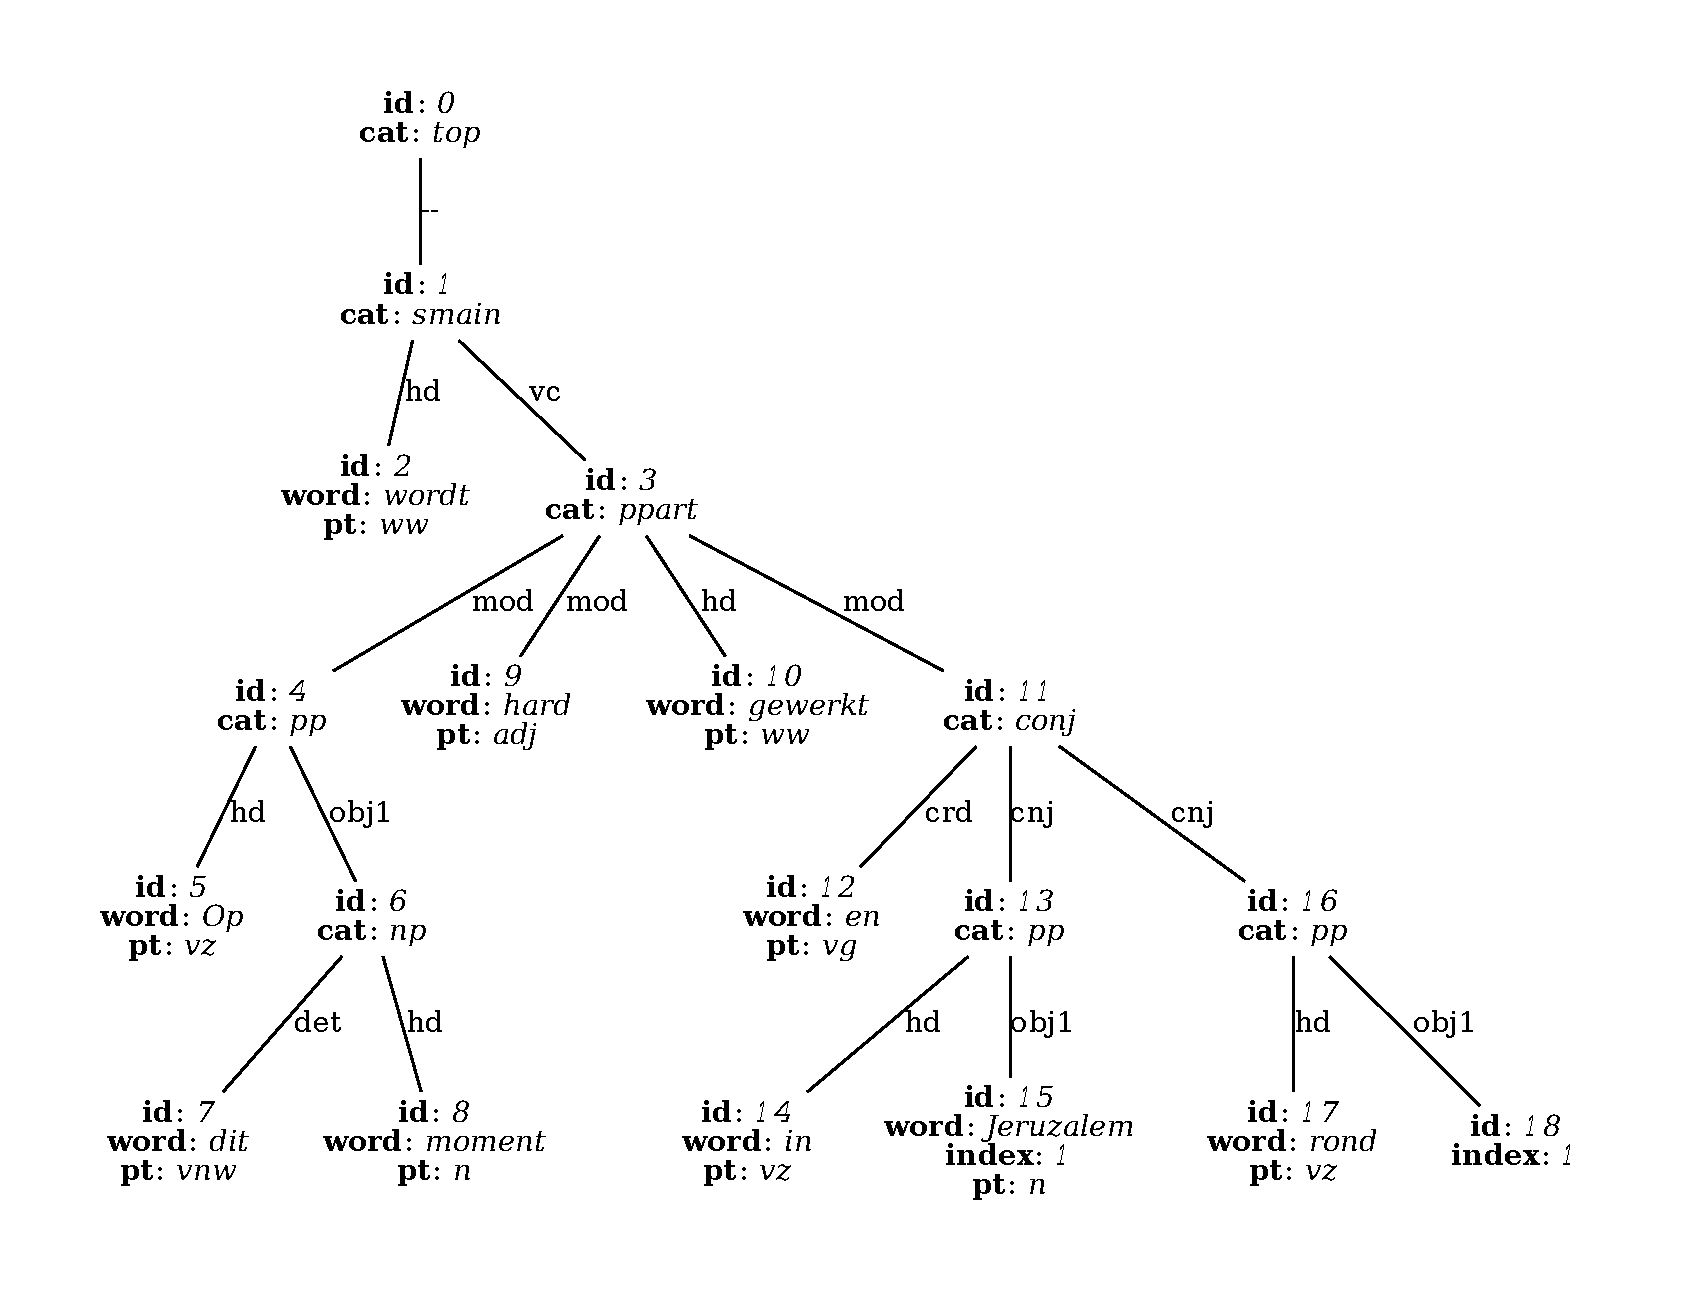
\includegraphics[width=1\textwidth,trim={1.25cm 0 1.25cm 0}, clip]{./prebuilt/parse_example.pdf}
	\lassycap
		{WS-U-E-A-0000000013.p.37.s.1}
		{Op dit moment wordt hard gewerkt in en rond Jeruzalem.}
		{At the moment there is hard work being done in and around Jerusalem.}
	\caption{Example Lassy graph. Note the identification of nodes 15 and 18 by a common index, marking the double use of \textex{Jeruzalem} as the direct object of prepositioal phrases 13 and 16.}
	\label{figure:example_lassy_tree}
\end{figure}

\begin{table}
	\centering
	\begin{tabularx}{0.925\textwidth}{@{}cccc@{}}
	      \textbf{Tag} & \textbf{Description} & \textbf{Frequency} (\%) & \textbf{Assigned Type}\\
	      \toprule
	      \multicolumn{4}{@{}c@{}}{Lassy Short POS Tags}\\
	      \midrule[0.005pt]
	      \textit{adj} & Adjective & 7.3 & \adj[s]\\
	      \textit{bw} & Adverb & 4.5 & \bw[s]\\
	      \textit{let} & Punctuation & 11.2 & \letter[s]\\
	      \textit{lid} & Article & 10.7 & \lid[s]\\
	      \textit{n} & Noun & 22.5 & \n[s]\\
	      \textit{spec} & Special Token & 3.5 & \np[s]\\
	      \textit{tsw} & Interjection & $<$0.1 & \tsw[s]\\
	      \textit{tw} & Numeral & 2.4 & \tw[s]\\
	      \textit{vg} & Conjunction & 4.2 & \vg[s]\\
	      \textit{vnw} & Pronoun & 6.5 & \vnw[s]\\
	      \textit{vz} & Preposition & 13.7 & \vz[s]\\
	      \textit{ww} & Verb & 13.2 & \ww[s]\\
	      \midrule[0.005pt]
	      \multicolumn{4}{@{}c@{}}{Lassy Phrasal Categories}\\
	      \midrule[0.005pt]
	      \textit{advp} & Adverbial Phrase & 0.6 & \adv[s]\\
	      \textit{ahi} & Aan-Het Infinitive & $<$0.1 & \ahi[s]\\
	      \textit{ap} & Adjectival Phrase & 2.1 & \adjp[s]\\
	      \textit{cp} & Complementizer Phrase & 3.3 & \cp[s]\\
	      \textit{detp} & Determiner Phrase & 0.2 & \detp[s]\\
	      \textit{inf} & Bare Infinitival Phrase & 4.7 & \infp[s]\\
	      \textit{np} & Noun Phrase & 36.7 & \np[s]\\
	      \textit{oti} & Om-Te Infinitive & 0.8 & \oti[s]\\
	      \textit{pp} & Prepositional Phrase & 23.2 & \pp[s]\\
	      \textit{ppart} & Past Participial Phrase & 4.2 & \ppart[s]\\
	      \text{ppres} & Present Participial Phrase & 0.1 & \ppres[s]\\
	      \textit{rel} & Relative Clause & 1.9 & \rel[s]\\
	      \textit{smain} & SVO Clause & 4.7 & \smain[s]\\
	      \textit{ssub} & SOV Clause & 0.8 & \ssub[s]\\
	      \textit{sv1} & VSO Clause & $<$0.1& \svi[s]\\
	      \textit{svan} & Van Clause & $<$0.1 & \svan[s]\\
	      \textit{ti} & Te Infinitive & 1.8 & \ti[s]\\
	      \textit{whq} & Main WH-Q & 0.1 & \whq[s]\\
	      \textit{whrel} & Free Relative & 0.2 & \whrel[s]\\
	      \textit{whsub} & Subordinate WH-Q & 0.2 & \whsub[s]\\
	      \textcolor{gray}{\textit{du}} & \textcolor{gray}{Discourse Unit} & \textcolor{gray}{2.6} & \textcolor{gray}{{\small n/a}}\\
	      \textit{mwu} & Multiword Unit & 5.9 & --\\
	      \textit{conj} & Conjunct & 5.7 & --
	\end{tabularx}
	\caption{Lassy POS tags and phrasal category labels, and corresponding atomic types. The \textit{du} category doesn't make its way to the extracted proofs, while \textit{mwu} and \textit{conj} don't have their own type.}
	\label{table:catset}
\end{table}

\begin{table}
	\centering
	\begin{tabularx}{0.925\textwidth}{@{}cccc@{}}
	      \textbf{Label} & \textbf{Description} & \textbf{Frequency} (\%) & \textbf{Modality}\\
	      \toprule
	      \textit{app} & Apposition & 0.8 & $\dbox{app}$\\
	      \textit{body} & WH-question Body & 0.1 & $\ddia{whbody}$\\
	      \textit{body} & Relative Clause Body &0.1& $\ddia{relcl}$\\
	      \textit{body} & Complementizer body & 2 & $\ddia{cmpbody}$\\
	      \textit{cnj} & Conjunct &4.3& $\ddia{cnj}$\\
	      \textit{crd} & Coordinator &1.8& --\\
	      \textit{crd} & Second Element of Correlative 	& $<$0.1 & $\ddia{cor}$\\
	      \textit{det} & Determiner &9.7& $\dbox{det}$\\
	      \textcolor{gray}{\textit{dlink}} & \textcolor{gray}{Discourse Link} & \textcolor{gray}{0.2} & \textcolor{gray}{{\small n/a}}\\
	      \textcolor{gray}{\textit{dp}} & \textcolor{gray}{Discourse Part} & \textcolor{gray}{0.8} & \textcolor{gray}{{\small n/a}}\\
	      \textit{hd} & Phrasal Head & 27.8 & -- \\
	      \textit{hdf} & Final Part of Circumposition & $<$0.1 & $\ddia{hdf}$\\
	      \textit{ld} & Locative Complement &0.5& $\ddia{ld}$\\
	      \textit{me} & Measure Complement &0.1& $\ddia{me}$\\
	      \textit{mod} & Modifier &16.4& $\dbox{mod}$\\
	      \textcolor{gray}{\textit{mwu}} & \textcolor{gray}{Multiword Part} & \textcolor{gray}{5.1} & \textcolor{gray}{{\small n/a}}\\
	      \textcolor{gray}{\textit{nucl}} & \textcolor{gray}{Nuclear Clause} &\textcolor{gray}{0.5}& \textcolor{gray}{{\small n/a}}\\
	      \textit{obcomp} & Comparison Complement &0.1& $\ddia{obcomp}$\\      
	      \textit{obj1} & Direct Object &10.8& $\ddia{obj1}$\\
	      \textit{obj2} & Secondary Object &0.2& $\ddia{obj2}$\\
	      \textit{pc} & Prepositional Complement &10.6& $\ddia{pc}$\\      
	      \textit{pobj1} & Preliminary Direct Object &$<$0.1& $\ddia{pobj1}$\\      
	      \textit{predc} & Predicative Complement &1.3& $\ddia{predc}$\\      
	      \textit{predm} & Predicative Modifier &0.1& $\dbox{predm}$\\      
	      \textcolor{gray}{\textit{sat}} & \textcolor{gray}{Satellite} & \textcolor{gray}{0.2} & \textcolor{gray}{{\small n/a}}\\
	      \textit{se} & Obligatory Reflexive Object &0.7& $\ddia{se}$\\      
	      \textit{su} & Subject &6.9& $\ddia{su}$\\
	      \textit{sup} & Preliminary Subject &$<$0.1& $\ddia{sup}$\\
	      \textit{svp} & Separable Verbal Participle &0.7& $\ddia{svp}$\\   
	      \textit{vc} & Verbal Complement &2.8& $\ddia{vc}$\\
	      \textit{tag} & Appendix &0.1& $\ddia{tag}$\\
	      \textit{whd} & WH-question Head &0.1 & --\\
	      \textit{rhd} & Relative Clause Head & 0.1 & --\\
	\end{tabularx}
	\caption{Lassy dependency labels, and corresponding modalities.
	Grayed out dependencies don't make their way to the extrated proofs.
	Heady dependencies don't get a modality.
	}
	\label{table:depset}
\end{table}

\begin{table}
	\centering
	\small
	\begin{tabularx}{1\textwidth}{@{}ccccc@{}}
	\textbf{Treebank} 	& \textbf{Contents}  & \textbf{Acronym} & \textbf{\# Sentences} & \textbf{\# Words}\\
	\toprule
	\textbf{DPC}		& Dutch Parallel Corpus 	& \fname{dpc} & {11\,716} 	& {193\,029}\\
	\addlinespace
	\addlinespace
	\textbf{Wikipedia} & Wikipedia Pages 			& \fname{wiki} & {7\,341} 	& {83\,360}\\
	\addlinespace
	\addlinespace
	\multirow{5}{*}{\textbf{WR-P-E}} 
						& E-magazines				& \fname{WR-P-E-C} 			& \multirow{5}{*}{14\,420} & \multirow{5}{*}{232\,631}\\
						& Newsletters				& \fname{WR-P-E-E}\\
						& Teletext Pages			& \fname{WR-P-E-H}\\
						& Web Sites					& \fname{WR-P-E-I}\\
						& Wikipedia					& \fname{WR-P-E-J}\\
	\addlinespace
	\addlinespace
	\multirow{10}{*}{\textbf{WR-P-P}} 
						& Books						& \fname{WR-P-P-B} 			& \multirow{10}{*}{17\,691} & \multirow{10}{*}{281\,424}\\
						& Brochures					& \fname{WR-P-P-C}\\
						& Guides \& Manuals		& \fname{WR-P-P-E}\\
						& Legal Texts				& \fname{WR-P-P-F}\\
						& Newspapers				& \fname{WR-P-P-G}\\
						& Periodicals \& Magazines	& \fname{WR-P-P-H}\\
						& Policy Documents			& \fname{WR-P-P-I}\\
						& Proceedings				& \fname{WR-P-P-J}\\
						& Reports					& \fname{WR-P-P-K}\\
						& Surveys					& \fname{WR-P-P-L}\\
	\addlinespace
	\addlinespace
	\multirow{3}{*}{\textbf{WS-U}}
						& Auto Cues					& \fname{WS-U-E-A}			& \multirow{3}{*}{14\,032} & \multirow{3}{*}{184\,611}\\
						& News Scripts				& \fname{WS-U-T-A}\\
						& Text for the Visually Impaired& \fname{WS-U-T-B}
	\end{tabularx}
	\caption{Breakdown of Lassy Small contents.}
	\label{table:lassy_contents}
\end{table}

\section{\AE thel}
The stage is set.
We need to devise an algorithm that accepts trees like the one of Figure~\ref{figure:example_lassy_tree} and spits out proofs of $\NLP_{\diamond,\bx}$.
Following our prior discussions, some assumptions need to be met before we get to even contemplate our approach.
First, we need a clear three-way partition of the set of dependency labels, so that each dependency relation marks either a head, a complement or an adjunct.
Further, we require that each dependency domain has exactly one head.
Finally, we must ensure that higher order phenomena reflected in secondary edges (or phantom nodes) are homogeneous so that they can be treated in a uniform way.
Unfortunately, these requirements are not always met; our first step is therefore to massage any rough edges with a series of transformations aimed at (i) harmonizing the input trees with the target logic and (ii) fixing inconsistent formattings and underspecified or otherwise incompatible annotations. 

\subsection{Taming Lassy}
\subsubsection{Edge Relabeling}
A phrasal annotation canonically contains a single head, a collection of complements (no more than one of each), and a collection of adjuncts (without any restriction on their plurality), where verbal, nominal and sentential domains differ in the the labels they may contain.
Deciding whether a dependency edge signifies a head, a complement or an adjunct requires little effort on our part, as the distinction has already been made.
The Lassy annotation manual specifies labels \{\textit{hd}, \textit{rhd}, \textit{whd}, \textit{cmp}, \textit{crd}, \textit{dlink}\} as heads of various kinds, \{\textit{det}, \textit{mod}, \textit{app}, \textit{predm}\} as adjuncts, and \{\textit{body}, \textit{cnj}, \textit{hdf}, \textit{ld}, \textit{me}, \textit{obcomp}, \textit{obj1}, \textit{obj2}, \textit{pc}, \textit{pobj1}, \textit{predc}, \textit{se}, \textit{su}, \textit{sup}, \textit{svp}, \textit{vc}\} as complements.
This is not a full partition of the set of dependency labels of Table~\ref{table:depset}, as several items fall in neither of the above bins -- more on that in a second.
First, we'll take on the less severe problem of standardizing the labels already categorized.

\paragraph{\textit{body}, but what kind of?}
A minor problem appears in the reuse of the \textit{body} label in three different contexts: as the body of a wh-question, a relative clause, or a complementizer.
This conflation is perfectly reasonable from Lassy's angle: in all three constructions, the head specifies the dependency (being either \textit{whd}, \textit{rhd} or \textit{cmp}) and selects for a subordinate clause with a gap that is practically agnostic to its external context.
This scheme backfires in our setup, due to heads not carrying their own annotation but rather imposing one on their complements -- if we keep the \textit{body} relation as is, the three different types of head would be indistinguishable.
Counteracting this is easy; we simply subcategorize the \textit{body} label according to the label of its head, giving rise to labels \textit{whbody}, \textit{relcl} and \textit{cmpbody}.
This doesn't have any intended consequences on the interal structure and typing of the complement, as its contents still has no premonition as to what diamond it will eventually be assigned.

\paragraph{\textit{det} or \textit{mod}?}
Lassy is occassionally inconsistent with the use of the determiner \textit{det} and modifier \textit{mod} labels in the nominal domain, marking either as the other in various contexts.
Examples include marking indefinite, demonstrative or possessive pronouns as modifiers, and, the other way around, marking numerals, names in genitive form, quantifiers and complex quantifying phrases as determiners -- but neither direction is strictly followed.
These annotations can at times result in a phrase with multiple determiners.
Despite determiners not being heads, the presence of multiple of them makes it hard to decide on a compositional structure as it poses the challenge of choosing one as the primary between them.
To impose the restriction of a single determiner per nominal domain and to standardize (some of the) inconsistencies, we uniformly cast the former to determiners and the latter to modifiers, using simple lexical filtering.
This results in a unique determiner per phrase (resolving constructions like \texttr{geen enkel}{no}, \texttr{de beide}{both}, etc.), and an elimination of complex determiner phrases.

\paragraph{Nominal and Verbal Domains}
Lassy uses the label \textit{hd} to refer to both the head of a matrix clause and to the head of a noun phrase.
To distinguish between the two, we relabel heads co-occurring with a determiner to \textit{np-head}.
This has no effect on our extracted types and proofs but shall help us formulate the extraction algorithm in a more transparent way.

\subsubsection{Non-Compositional Annotations}
Despite its admittedly high quality, Lassy has not been built with an inherent focus towards compositionality.
This reflects in some not so uncommon exceptions to the canonical phrasal annotation that \textit{de facto} necessitate some global concessions and adaptations, and some local emergency measures, ranging from targeted transformations in the best case, to occassionally just giving up on a sample in the worst.
The biggest problem that we are faced with right off the bat is the abundance of vague, general purpose annotation schemes to convey non-compositional structures.
These come in two flavours -- discourse level annotations, and multiword phrases.

\begin{figure}
	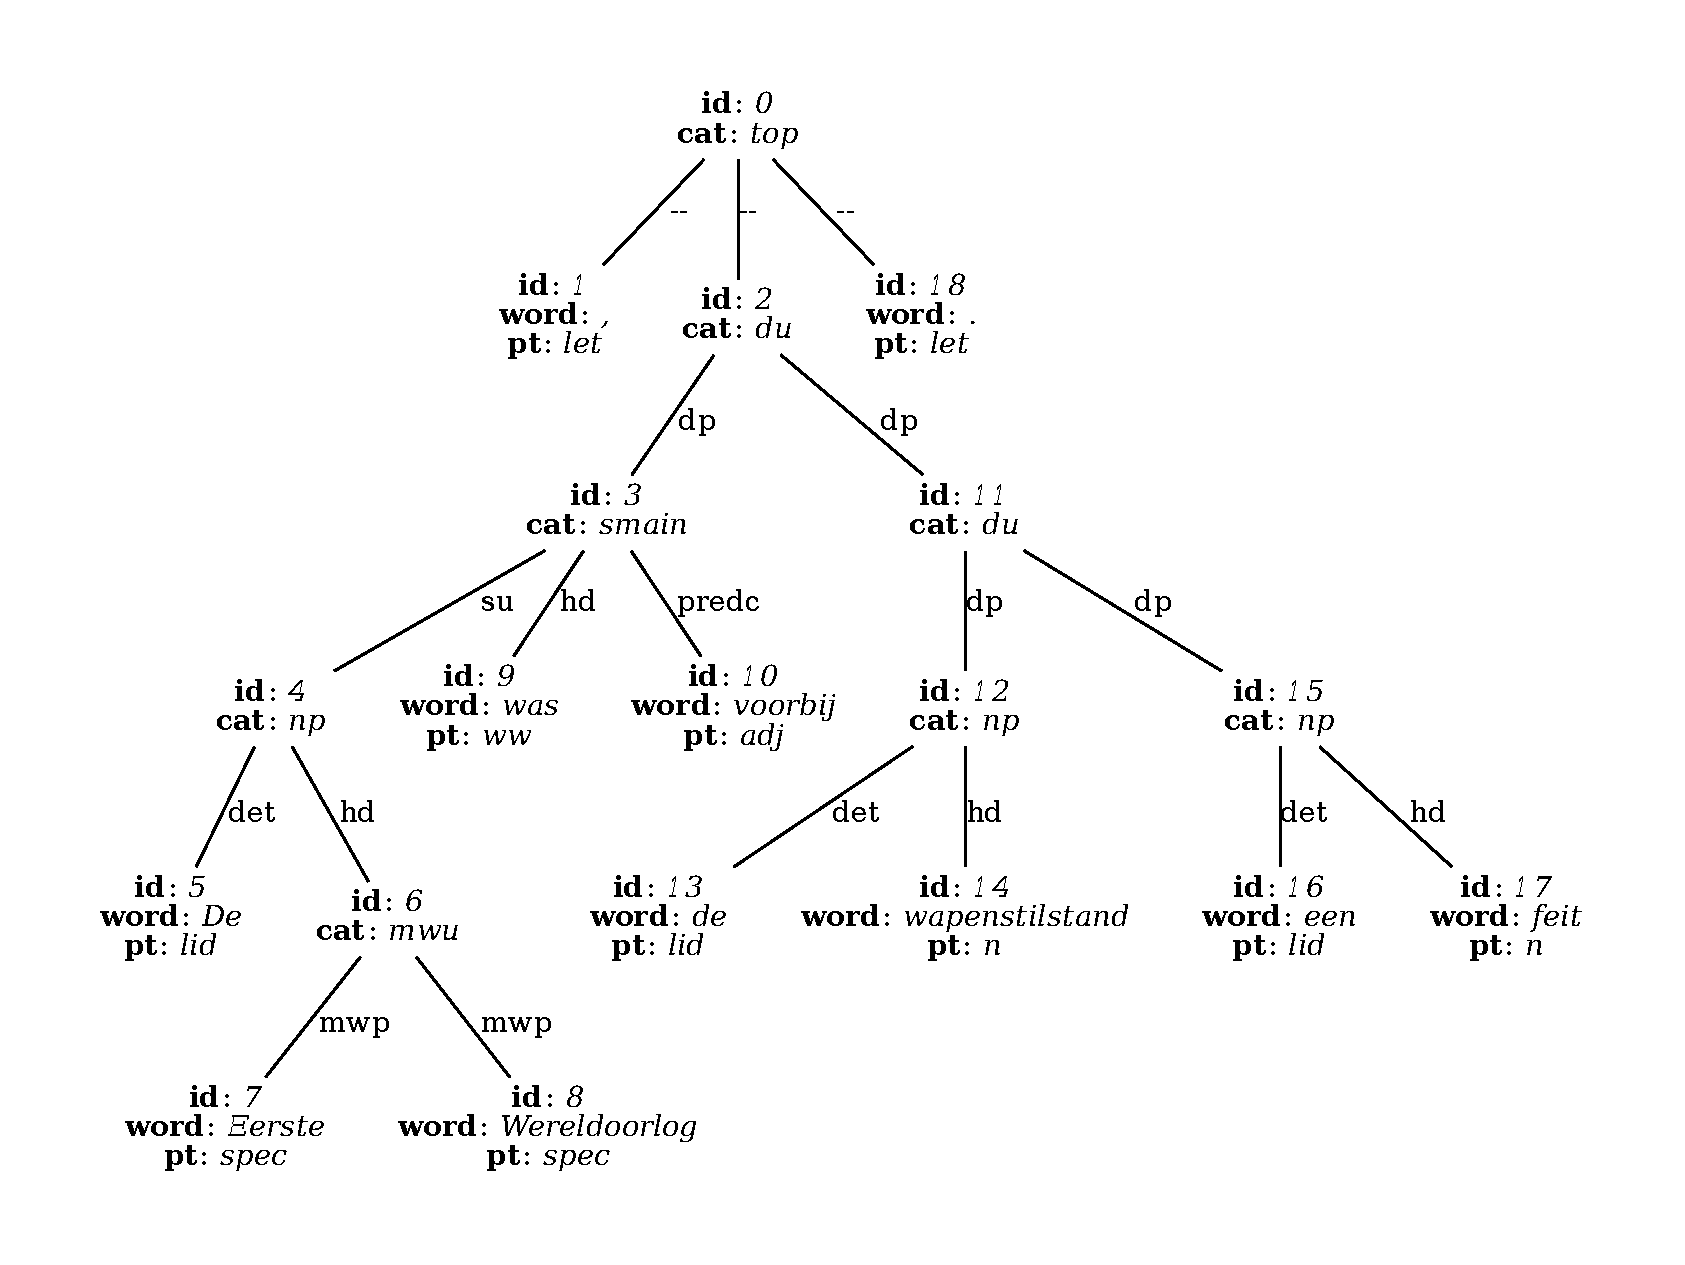
\includegraphics[width=1\textwidth,trim={1.25cm 0 1.25cm 0}, clip]{./prebuilt/du_mwp_example.pdf}
	\lassycap
		{wiki-4941.p.4.s.2}
		{De Eerste Wereldoorlog was voorbij, de wapenstilstand een feit.}
		{The first world war was over, the armistice a fact.}
	\caption{Example Lassy graph showcasing non-compositional annotations.}
	\label{figure:du_mwp_example}
\end{figure}

\paragraph{Discourse Level Annotations}
Discourse level annotations are materialized by dependencies \textit{dlink}, \textit{dpart}, \textit{nucl} and \textit{sat}, used in a catch-all fashion in place of an actual syntactic analysis.
In the example of Figure~\ref{figure:du_mwp_example} the two sentences are analyzed as ``discourse parts'' of a single ``discourse unit'' rather than matrix clauses conjoined by the comma -- with some goodwill we could let that slide, but that same strategy is internally applied within the second sentence (apparently a ``discourse unit'' rather than a sentence), thus avoiding a proper syntactic justification for the elided verb. 
Unfortunatey, there is no algorithmic way to mend these pretend annotations, in part due to their wildly general use, but mostly due to the fact they give us nothing to work with.
This phenomenon is unpleasantly common; discourse level annotations sum up to about 2\% of the total dependency edges in the corpus, and are present in some 11\,700 samples, polluting a hard to ignore 18\% of the dataset.
In order not to lose all the precious samples in their totality, we take the more conservative approach of simply pruning the problematic edges rather than discard the entire tree.
The subtree underneath each cut is subsequently rooted as an independent sample, sprouting an array of smaller samples from the larger unusuable original; in the example under scrutiny, we end up with three samples rooted at nodes 3, 12 and 15.
Albeit being a sensible solution in terms of data preservation, this has the unavoidable downside of \textit{a priori} breaking the alignment between the source corpus and the collection of proofs to be.
In order to facilitate some level of back-and-forth matching, the new samples inherit the sample name of their origin and are distinguished between one another by a suffix corresponding to the identifier of their root node.

The pruning might sound easy on paper but proves tricky in certain regards.
Lassy by default provides no annotations for punctuation symbols, which are instead attached to a conventional ``top'' node with an unlabeled edge.
By truncating trees naively, we'd be dropping punctuation that might be necessary for a phrase to remain grammatical or otherwise prove useful in the provision of a proper derivation.
Internal commas, for instance, could be the key to constructing a conjunction, whereas final punctuation might be crucial in deciding the phrasal type, motivating their reinstation.
Including internal and right-adjacent punctuation only, however, carries the risk of upholding only one end of circumfixing punctuations like parentheses or brackets, accidentally turning a phrase ungrammatical.
The heuristic solution is to iteratively expand a truncated subtree by attaching any internal or peripheral punctuation marks, excluding opening brackets from the right edge and closing brackets and sentence-final punctuation from the left edge.
To homogenize trees (truncated or otherwise), punctuations are displaced from the ``top'' node to the top-most node that carries an actual syntactic category label -- the latter serves as the new tree's root.

The next issue to address is the occasional disconnect between a phantom node and its material counterpart as a result of pruning.
To avoid trees with floating nodes, we check whether phantoms in the pruned tree can access their material counterparts.
When that's not the case, the phantom node is substituted by a copy of the material one, and, in the event of it being phrasal, the entire tree that lies underneath it.
The process is repeated (to circumvent the possibility of adding a new floating node when fixing the first) until a fixpoint is reached.
The result is the possibile duplication of lingustic material among different prunings (i.e. a subtree that occurred once in the original Lassy sample can sometimes be found in more than one of the processed samples).

\begin{figure}
	\centering
	\begin{subfigure}[b]{0.65\textwidth}
		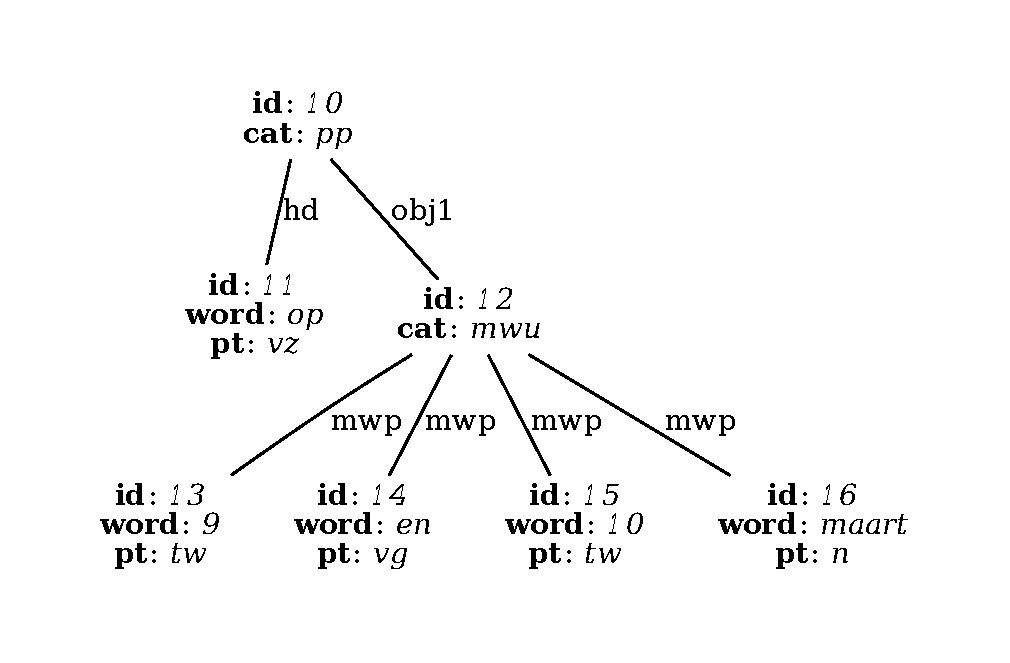
\includegraphics[width=1\textwidth,trim={1.5cm 1.5cm 1.5cm 1.5cm}]{./prebuilt/date_before.pdf}
		\caption{Before.}
	\end{subfigure}\\[\midsep]
	\begin{subfigure}[b]{0.55\textwidth}
			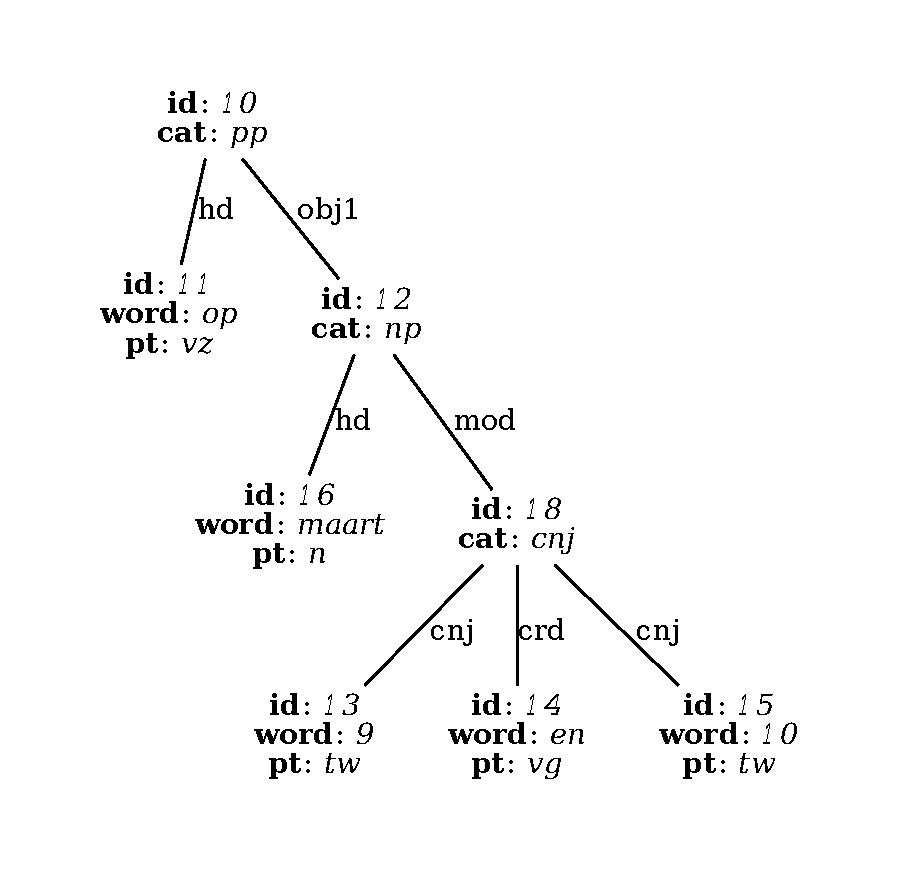
\includegraphics[width=1\textwidth,trim={1.5cm 1.5cm 1.5cm 1.5cm}]{./prebuilt/date_after.pdf}
			\caption{After.}
	\end{subfigure}\\[\smallsep]
	\lassycap
		{WR-P-P-I-0000000242.p.16.s.2~\textnormal{(excerpt)}}
		{...op 9 en 10 maart...}
		{...on March 9 and 10...}
	\caption{Reannotating a date expression containing a conjunction.}
	\label{figure:mwu:datetime}
\end{figure}

\begin{figure}
	\centering
	\begin{subfigure}[b]{0.85\textwidth}
		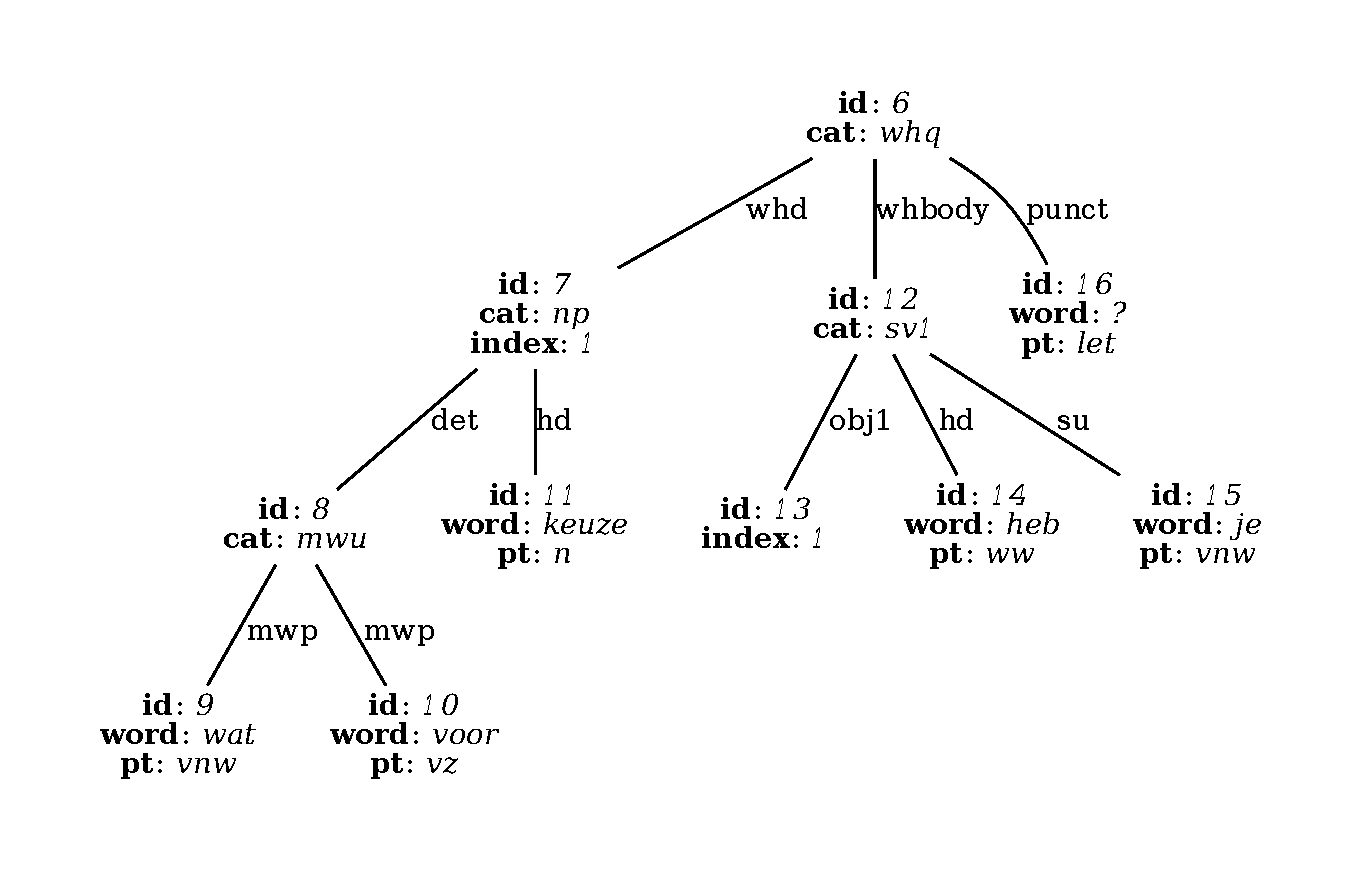
\includegraphics[width=1\textwidth,trim={1.5cm 1.5cm 1.5cm 1.5}]{./prebuilt/watvoor_before.pdf}
		\caption{Before.}
	\end{subfigure}\\[\midsep]
	\begin{subfigure}[b]{0.75\textwidth}
			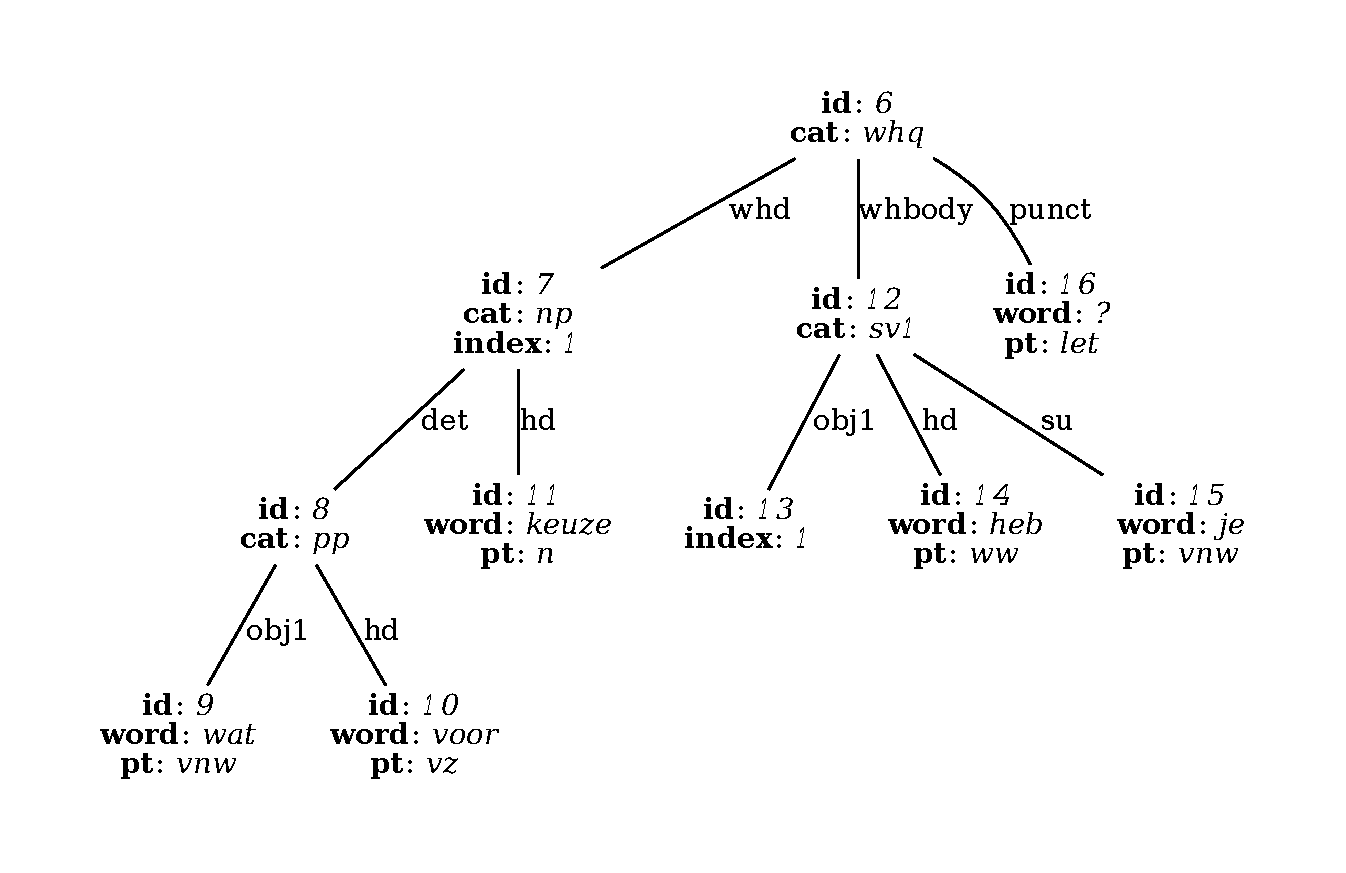
\includegraphics[width=1\textwidth,trim={1.5cm 1.5cm 1.5cm 1.5cm}]{./prebuilt/watvoor_after.pdf}
		\caption{Before.}
	\end{subfigure}\\[\smallsep]
	\lassycap
		{WR-P-P-H-0000000039.p.8.s.3(6)}
		{wat voor keuze heb je?}
		{what kind of choice do you have?}
	\caption{Rennotating an erroneously analyzed interrogative.}
	\label{figure:mwu:watvoor}
\end{figure}

\paragraph{Multiword Phrases}
Another common pain point is the prominence of multiword phrase annotations, indicated in Lassy by the \textit{mwu} dependency.
Multiword expressions are a pervasive pest from the shadowy realms between lexicon and syntax.
They can be categorized as being either (i) morphosyntactically fixed or (partially) productive expressions that deviate from the expected compositional meaning, or (ii) just compositional expressions that have an idiosyncratic frequency.
In all but the first case and regardless of their semantic use, they are not necessarily without internal structure.
The criteria of what constitutes a multiword phrase and what doesn't are somewhat muddy, subjective and not clearly motivated.
The example of Figure~\ref{figure:du_mwp_example} claims that \texttr{Eerste Wereldoorlog}{first world.war} is one, for instance -- eliciting the questions of whether expressions like the \textex{third/current/last/next world war} are also instances of a multiword phrase, and, if so, where the line is drawn (if at all).
Anyway, multiword expressions are bad, but what's really bad is how overindulgent Lassy is with their use, which feels more like a free pass at disclaiming any responsibility of actually providing an analysis: a preposterous 5.9\% of all composite phrases are labeled as being multiword expressions.

Multiword phrases are not an impassable roadblock; they can be tackled by relaxing the lexicalist word-to-type restriction, i.e. allowing entries in the lexical dictionary to be arbitrary strings rather than words.
This is indeed the approach we'll follow, but only after having salvaged however many of the missing annotations as we can.
Doing so is in our best interest: it will reduce the lexicon's load and provide us with a collection of annotations that are easier to generalize from.
Generating structure out of thin air is of course impossible, but several existing patterns are amenable to an automatic reannotation.

A first filter can tell us whether a word is a numeral or measure by inspecting its part of speech assignment.
Two numerals separated by a coordinator make for a complex numeral, in which case a new tree can be instantiated, with the coordinator and the two numerals as its daughters; the first marked as a coordinator, the other two as conjuncts.
A numeral, complex or singleton, adjacent to a quantity denoting noun (like \texttr{paar}{pair}, \texttr{honderd}{hundred}, \texttr{duizend}{thousand}, etc.), a unit of measurement (like \texttr{kilo}{kilogram}, \texttr{eur}{euro}, etc.) is cast into a modifier, and the noun is cast into a head.
In a similar vein, a tiny parser is employed to analyze expressions of time and date; it follows a binarization scheme that assigns headedness to the more general part of a datetime expression (i.e. year over month over day), and analyzes the rest as a modifier with internal structure; an example is presented in Figure~\ref{figure:mwu:datetime}.

On the lexical side of things, some expressions tend to default to a multiword annotation despite not being one -- clearly an artifact of Alpino's rule-based parser that was never corrected in the manual verification stage.
These are for the most part prepositional phrases (like \texttr{ten noorden van}{north of}, \texttr{met uitzondering van}{except for}, etc.), which are caught and reanalyzed by having the genitive-substitute \textex{van} attach to the modified noun (as consistently done otherwise throughout Lassy), which the remainder of the expression consumes as a direct object.
More problematic is the occasional mischaracterization of the interrogative \texttr{wat voor}{what kind of}, where the preposition \texttr{voor}{for} is analyzed as part of a multiword expression together with a phantom node coindexed with the pronoun \texttr{wat}{what}.
These are also caught and corrected, as in the example of Figure~\ref{figure:mwu:watvoor}; the preposition is reannotated as being the head of a prepositional phrase selecting for a direct object, that being the afforementioned phantom node.
Other, less severe, cases include the mislabeling of nationality adjectives (like \texttr{afrikaans}{Afrikan}, \texttr{europees}{european}, etc.), which are recast as modifiers of the noun they were merged with.
For consistency, punctuations originally analyzed as multiword parts (presumably so as not to break phrasal contiguity) are instead pushed to the topmost root.

These minor changes suffice to cut down the frequency of multiword expressions to a more manageable 4.5\% (an overall reduction of 25\%).
Unresolved expressions have their parts merged into a single node; the resulting node gets a new syntactic label, that being the most common part of speech tag of the merged units (with a bias towards \textit{n} or \textit{np}, if either is present in the parts).
The goal is to contain the effect of multiword annotations within their own phrasal boundaries (i.e. to avoid functors higher in the tree from selecting for \smallgtype{mwu}-typed arguments).
In the case of a multiword phrase consisting solely of phantom parts, the merged phrase also gets assigned an index and associating it to its material counterpart.

\subsubsection{There Can Be Only One (Head)}
Having dealt with structureless structures, the next thing to tackle are subtrees that fail to elect a single head, falling to civil war (when multiple nodes compete for the role) or rising to anarchy (when all relinquish it).
Here, we'll need to assume the interventive role of a self-appointed stabilizing force, and take it upon ourselves to reinstate normalcy (read: we'll assign a single head of our own choice).
The culprit behind both cases is always a conjunction, canonically containing a number of conjuncts (labeled \textit{cnj}) and a single coordinator (labeled \textit{crd}).
Exceptionally, we may have an instance of a so-called \textit{correlative conjunction}, where two words jointly perform the role of the coordinator (e.g. \texttr{zowel ... als}{as much ... as}, etc.).
We resolve this by changing the label of the second coordinator (in terms of left-to-right sentential precedence) to \textit{cor} (for correlative), which we will later treat as a complement.
Otherwise in the second case we have an arrangement of conjuncts with no coordinator in between.
In reality, the conjunction is licensed by a punctuation symbol (usually a comma, but sometimes a dash or an ampersand), which, being a punctuation, has gone under Lassy's radar.
We heuristically resolve this by first locating any occurrence of a single punctuation infixed between headless conjuncts, relocating it to its rightful place, and assigning it a \textit{crd} label; see Figure~\ref{figure:p2crd} for an example.

\begin{figure}
	\centering
	\begin{subfigure}[b]{0.85\textwidth}
		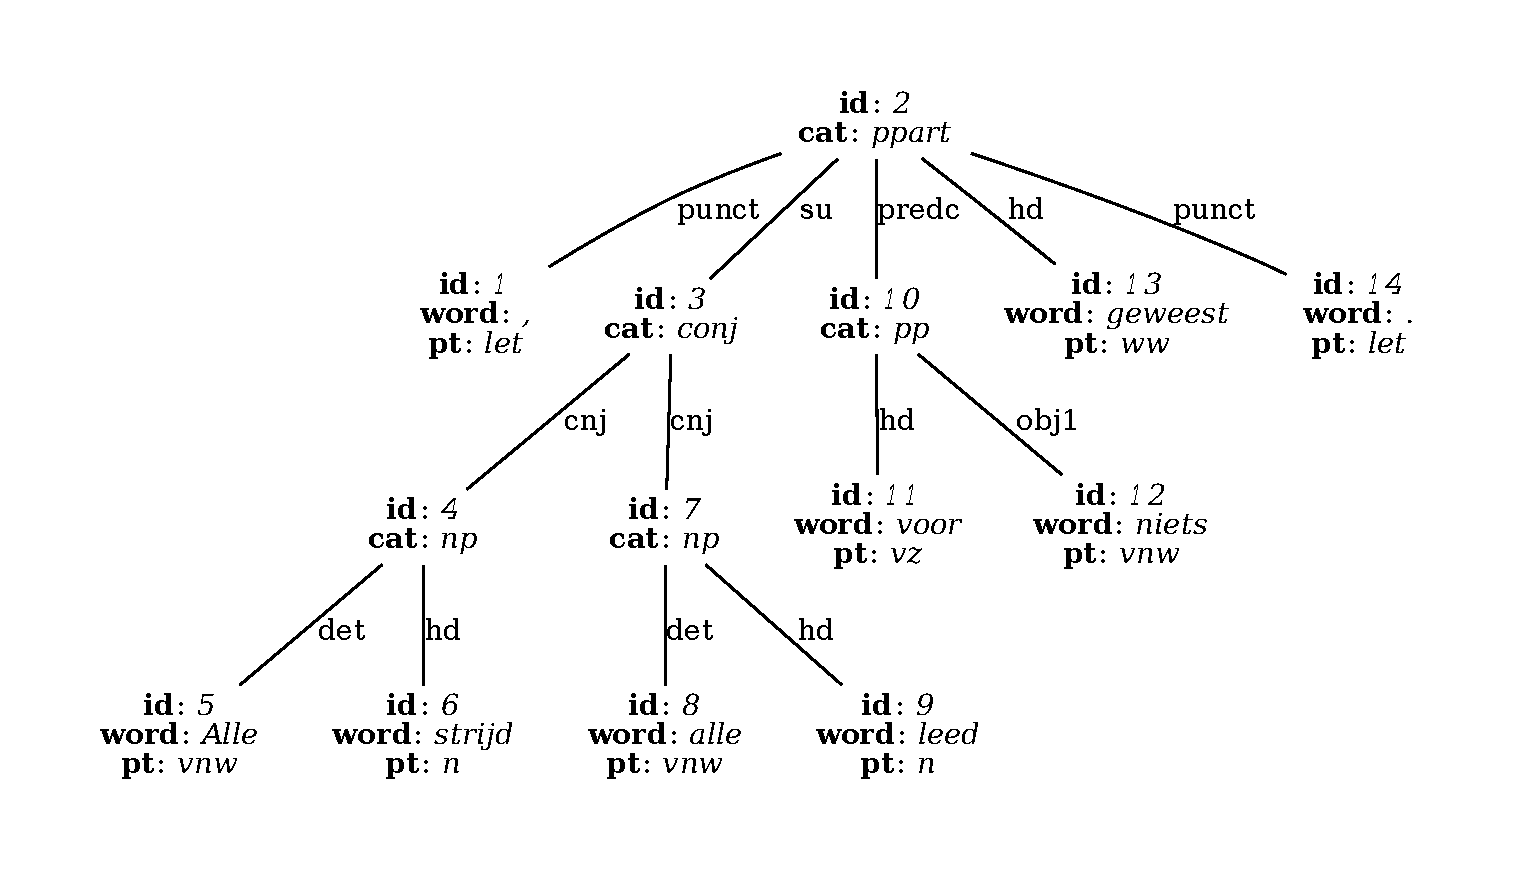
\includegraphics[width=1\textwidth,trim={1.5cm 1.5cm 1.5cm 1.5cm}]{./prebuilt/p2crd_before.pdf}
		\caption{Before.}
	\end{subfigure}\\[\midsep]
	\begin{subfigure}[b]{0.85\textwidth}
			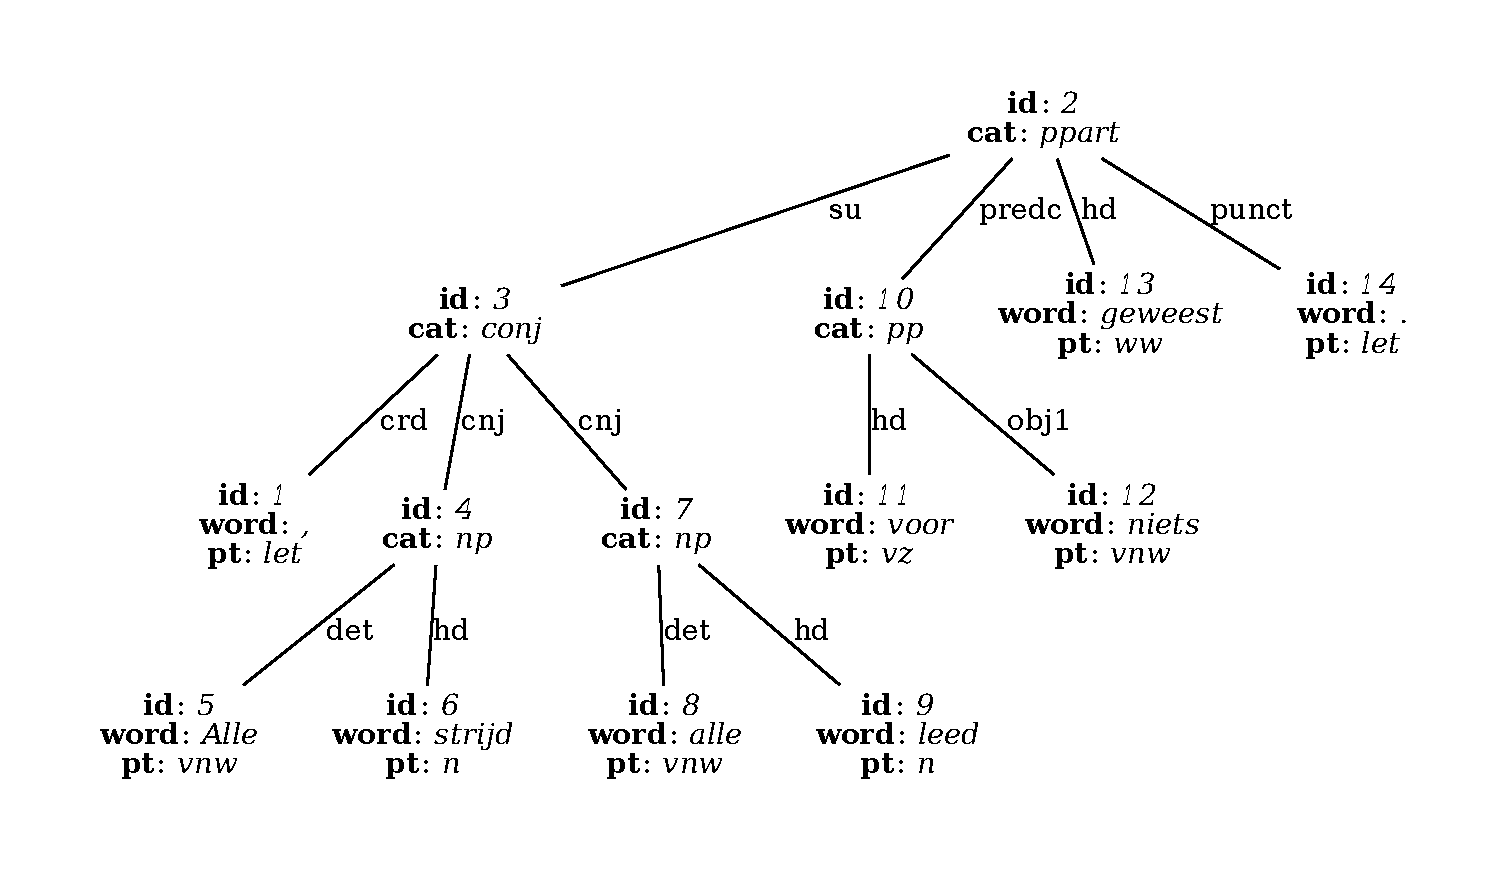
\includegraphics[width=1\textwidth,trim={1.5cm 1.5cm 1.5cm 1.5cm}]{./prebuilt/p2crd_after.pdf}
			\caption{After.}			
	\end{subfigure}\\[\smallsep]
	\lassycap
		{WR-P-E-I-0000050381.p.1.s.704(2)}
		{Alle strijd, alle leed voor niets geweest.}
		{All the struggle, all the suffering were for nothing.}
	\caption{Reannotating a headless conjunction.}
	\label{figure:p2crd}
\end{figure}

\subsubsection{Phrasal Restructuring}
Other than the incompatibilities detailed so far, some Lassy annotations are suboptimal for the target logic in specifying a phrasal structure that we want to treat differently than prescribed.
Such cases are treated by automatically adjusting the phrasal structure to one we are happier with.
Since these adjustments involve removing or establishing new subtrees and edges, we run the risk of accidentally removing the material tree that grounds a set of phantom nodes sharing the same index.
As a safety measure, we first enforce the convention that the most shallow occurrence of a node should correspond to a material tree.

\begin{figure}
	\centering
	\begin{subfigure}[b]{0.75\textwidth}
		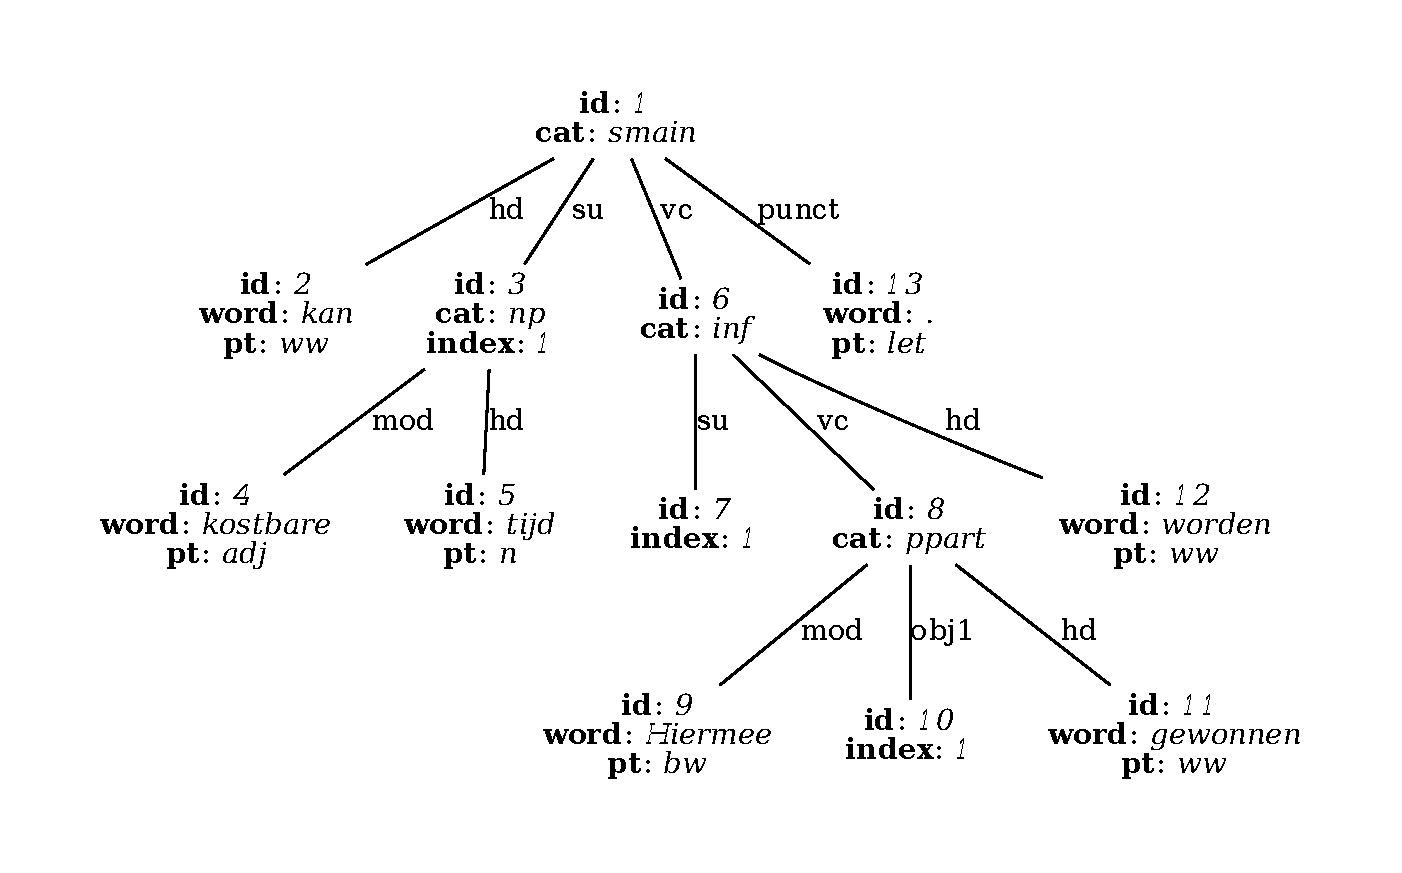
\includegraphics[width=1\textwidth, trim={1.5cm 1.5cm 1.5cm 1.5cm}]{./prebuilt/ua_before.pdf}
		\caption{Before.}
	\end{subfigure}\\[\midsep]
	\begin{subfigure}[b]{0.75\textwidth}
			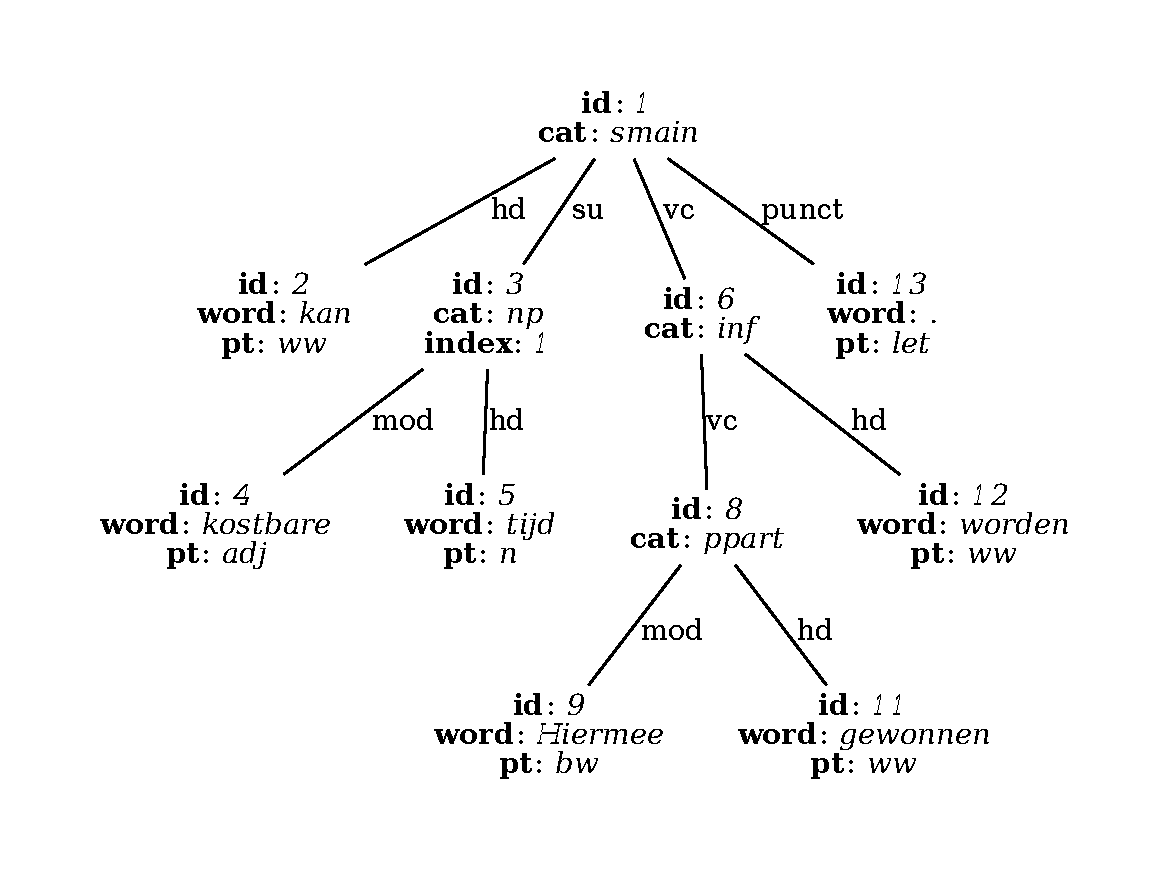
\includegraphics[width=1\textwidth,trim={1.5cm 1.5cm 1.5cm 1.5cm}]{./prebuilt/ua_after.pdf}
		\caption{After.}			
	\end{subfigure}\\[\smallsep]
	\lassycap
		{dpc-gaz-001006-nl-sen.p.52.s.4(1)}
		{Hiermee kan kostbare tijd gewonnen worden.}
		{Precious time can be won with this.}
	\caption{Removing the understood arguments from an infinitive and the participle nested within it.}
	\label{figure:ua}
\end{figure}

\paragraph{(Mis)understood Arguments}
Lassy treats the non-finite verbal forms (participles and infinitives) as verbal elements proper, selecting for all the arguments their finite counterparts would.
Obviously, participles used for the passive or the perfect and infinitives in verbal complements cannot possibly find all these arguments, some being located in higher levels of the dependency graph.
To resolve this, Lassy opts for establishing phantom nodes coindexed with the so-called understood argument.
The more non-finites in the path between the one under scrutiny and the top level clause, the more phantom nodes are inserted.
These nodes are purely semantic in nature, and no syntactic item allows for the consecutive duplication of material they call for.
As such, they have no place in the compositional structure we seek to extract, and we have the moral right to cast them away.%
	\footnote{Funnily, our recurring complaint with Lassy so far has been that it gives us too little. 
	This time around, it gives us too much.}
Concretely, we look for any edge with adependency label normally reserved for a nominal complement (i.e. \textit{su}, \textit{obj1}, \textit{obj2}, \textit{sup}, \textit{pobj}) pointing to a phantom node, such that any of its non-immediate ancestors is a sentential clause with an outgoing edge pointed to a node of the same index.
Edges caught in our web are deleted, as are any nodes left floating; see Figure~\ref{figure:ua} for an example.
This transformation incurs a loss of semantic coindexing, which anyway is irrelevant to us: it's up to lexical semantics entries to decide what arguments they have, how their slots are filled, and how these are propagated and updated down the sentence.
Other than this coindexing, it will soon be made apparent that no meaningful function-argument structures are actually lost by this erasure.


\begin{figure}
	\centering
	\begin{subfigure}[b]{0.75\textwidth}
		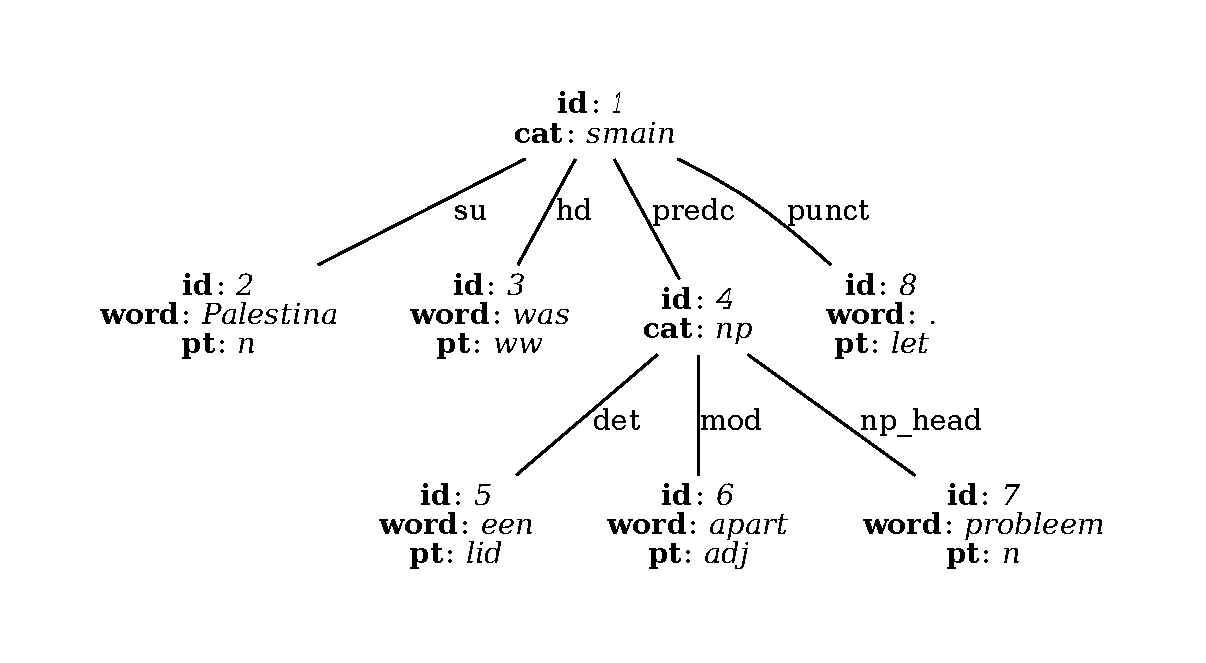
\includegraphics[width=1\textwidth, trim={1.5cm 1.5cm 1.5cm 1.5cm}]{./prebuilt/prenom_before.pdf}
		\caption{Before.}
	\end{subfigure}\\[\midsep]
	\begin{subfigure}[b]{0.75\textwidth}
			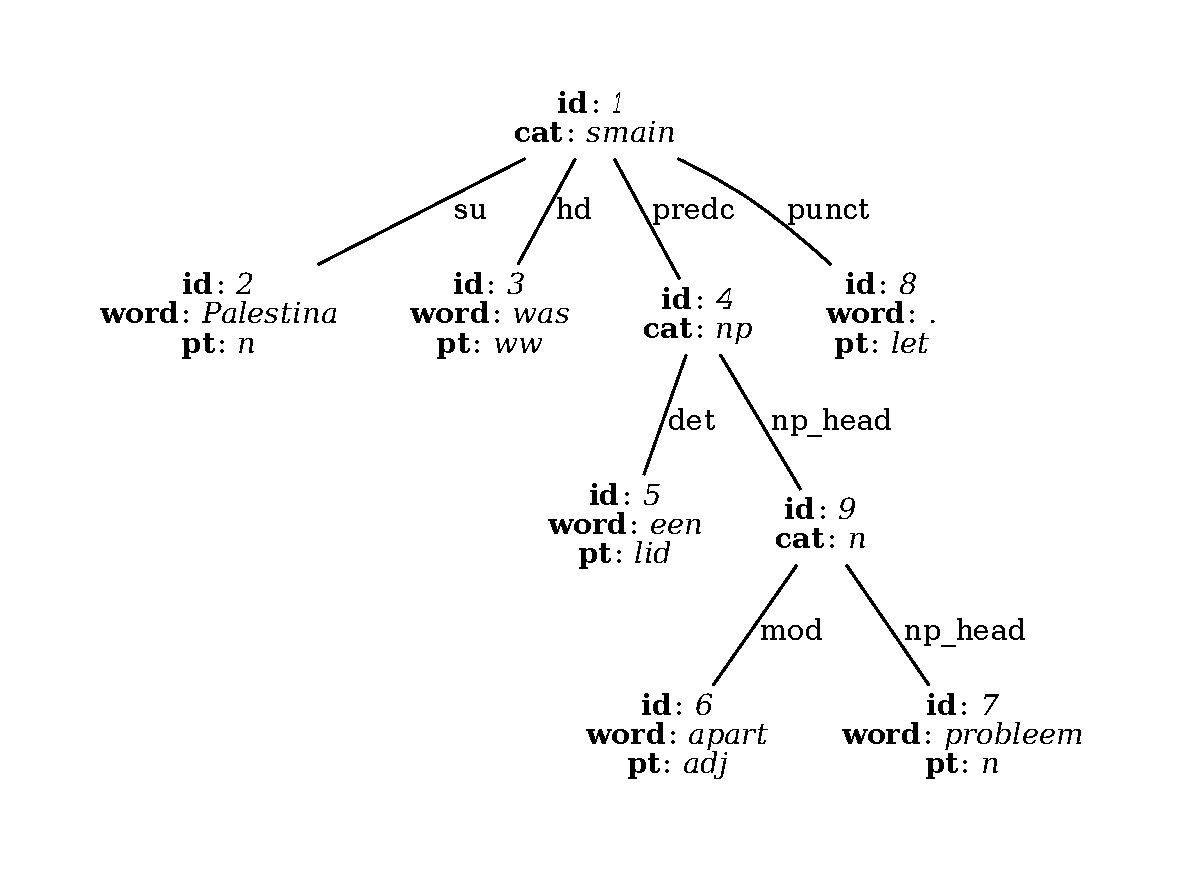
\includegraphics[width=1\textwidth,trim={1.5cm 1.5cm 1.5cm 1.5cm}]{./prebuilt/prenom_after.pdf}
		\caption{After.}
	\end{subfigure}\\[\smallsep]
	\lassycap
		{WR-P-E-I-0000051928.p.1.s.140(1)}
		{Palestina was een apart probleem.}
		{Palestine was a separate problem.}
	\caption{Inserting an intermediate layer for nominal modification.}
	\label{figure:prenom}
\end{figure}

\paragraph{Modifier Scope}
Unlike complements, adjuncts in Lassy are not limited to one occurrence per unique label.
In other words, they are attached in parallel to the phrasal domain they are part of, rather than recursive paired in a binary fashion to the node they modify or determine.
We managed to cheat our way around multiple determiners so as to avoid any conflicts of priority, but the same lexical strategy does not apply to modifiers.
Since Lassy abstains from taking a stance on what the order of modifier attachment is, and sees no distinction between modifying a phrase or its head, we are forced to by and large adopt the same strategy.
Exceptionally in the nominal domain, we have the option of imposing structure based on word order alone.
That is, we can distinguish between a noun and a noun phrase modifier depending on where the modifier is located: a modifier that occurs before the determiner must modify the entire phrase, whereas a modifier that occurs between the determiner and the head noun must modify the noun alone; see Figure~\ref{figure:prenom} for an example.
This simple heuristic is as as far as we can get, but it will help homogenize our extracted proofs and types by (i) aligning function application order and word order and (ii) alleviating any unecessary typing tension between \smallgtype{np} and \smallgtype{n} modifiers.

\paragraph{Ellided Constituents}
Other than non-finite verbal arguments, shared indexing is primarily employed by Lassy to indicate an omission of linguistic material in ellipses.
The scheme Lassy employs presents the material version of a ``shared'' tree (be it a deep structure or a singleton node) in the first conjunct daughter of an elliptical conjunction, and a phantom copy of it in each subsequent sister.
We alter this by pushing the material node to the top-level of the conjunction%
		\footnote{In the case of nested conjunctions, we stop at the first node assigned the \textit{conj} syntactic category that is an ancestor of \textit{all} phantom nodes of the same index and dependency.}
(i.e. as a sibling to all conjuncts), and substituting the gap left behind by a new phantom node of the appropriate index.
This will facilitate the easier typing of conjunctions later on.

\paragraph{Unary Pipes}
The movements and erasures performed can sometimes lead to ``pipes'' of unary trees.
We resolve these by removing any intermediate nodes and establishing a new edge from the source of the pipe to its end, inheriting the label of the edge that would previously appear first.

\paragraph{Labelless Conjunctions}
The \textit{conj} label, used as an umbrella category to classify all conjunctions, carries the same risk as the \textit{mwu} label, namely of polluting the functional type assignments of phrases outside the conjunction itself with a generic, multi-purpose argument type.
We resolve this exactly like before, namely by conducting a majority voting over the categories of all conjunct siblings and propagating the elected category upwards to the conjunction node, prioritizing noun phrases over nouns over everything else in orderto account for nominalization.

\paragraph{Raising Nouns}
Bare nouns are assigned the \textit{n} part of speech regardless of whether they need (or occur with) a determiner to occupy a verbal argument position.
To circumvent (to the extent possible) a combinatorial explosion of meaningless \smallgtype{n} and \smallgtype{np} argument variations, we alter the part of speech assignment of \textit{n} nodes that are not roofed under a \textit{np} from the former to the latter.
As we will soon see, this will alter the type assignment of these nodes, in analogy to an implicit and contextual lexicalization of an explicit noun raising rule.

% \todo : ad hoc transformations

\subsection{Proving Lassy}
With our transformations in place, the subdued corpus should be ripe for our proof extraction algorithm.

\subsubsection{Proof Charming}
The extraction is built around a tiny DSL written in Python, which allows one to formulate, represent and traverse valid proofs of \NLPplus.
By invoking the DSL while traversing the dependency tree of a Lassy sample, the extraction algorithm dynamically constructs a natural deduction proof, translating tree patterns into meta-theoretical proof operations.
Internalizing the syntactic validity assertions of \NLPplus{} is a costly procedure, both in terms of processing overhead and of maintainance effort required, especially considering how unconducive the language is to formal rigor.
On the other hand, it serves to eliminate the need for asynchronously interfacing with some external checker, and provides a formal guarantee that whatever the extraction algorithm produces is \textit{correct by construction}: any syntactic missteps will be caught on the spot and raise an exception.
As a bonus, the system can (and will) find use outside the scope of the extraction, as a representational intermediary for parsing and proof representation.
Detailing the specifics behind the implementation shouldn't be our main concern here; it suffices to know it exists and runs as a constant safety belt in all that follows.
If for whatever reason you enjoy watching people try to beat types into Python, you can take at a look at Appendix~\ref{sec:python_impl} (not for the faint of heart).

\subsubsection{Parameters}
We start by declaring our basic necessities.
First, a translation table (or function) that maps part of speech tags and syntactic category labels to types, used to provide non-contextual type assignments to lexical nodes and phrases.
The translation table currently in use is depicted in Table~\ref{table:catset}; it maps strictly to atomic types and takes most of the categorial labels at face value, mapping each of them to a unique image%
\footnote{It basically just converts italics to smallcaps.}.
Exceptionally, the \textit{spec} tag is cast into \smallgtype{np}, as the tag is (inconsistently) used as a generic annotation for places, persons, events and the like.
The codomain of the translation is in our case coincident with our logic's set of propositional constants, $\propcon$.
As hinted at earlier, the extraction is \textit{parametric} to this translation: the domain can be any of the sets of lexical tags Lassy provides access to, and the codomain is by no means restricted to atomic types.
This allows an easy adaptation to morpologically informed types, or a transition to an expanded theory (e.g. one that includes subtyping, additional axes of modal decorations, etc.). 
In principle, this can also allow a re-incorporation of implicit arguments for non-finite verbal forms, but doing so would not amount to much: as promised earlier, these are already trivially recoverable by a simple morphism (readily applicable on the extracted proofs) that sends non-finite forms to the desired complex types (immediate return on investment for taking source labels at face value).
In any case, the translation induces a function that naively tells us for each node what type the translation table prescribes to its part of speech tag (if lexical), syntactic category (if phrasal) or the correspond translations of its material counterpart (if phantom).

Then, we need an equivalence relation on the set of dependencies so as to partition it into heads, adjuncts and complements -- each non-head dependency is translated into a modal label, the union of which (together with the extraction modality) forming the set of modalities $\deps$.
For the set of dependencies, we also need a strict partial order, serving to impose an informal ordering of the arguments of a multi-argument functor.
With this, we avoid the responsibility of having to explicitly argue about an equivalence between argument order variations of the same head function: each complement will have a distinct modal decoration that decides how strongly it is attracted to the end result, yielding a canonical form for all types we'd be faced with (given the uniqueness of complements restriction).
This is reminiscent of the notion of a \textit{obliqueness hierarchy}~\cite{dowty1982grammatical}, which we can in fact use to produce some linguistically sensible types.
From more to least oblique, we have: \textit{svp}\textgreater\textit{obcomp}\textgreater\textit{vc}\textgreater\textit{me}\textgreater\textit{ld}\textgreater\textit{hdf}\textgreater\textit{pc}\textgreater\textit{se}\textgreater\textit{obj2}\textgreater\textit{predc}\textgreater\textit{obj1} \textgreater\textit{pobj1}\textgreater\textit{su}\textgreater\textit{sup}.

\subsubsection{Tree Patterns}
The algorithm takes the form of a proof assignment function, responsible for casting a local tree structure into a corresponding natural deduction proof.
The function is recursively called in a top-down fashion, its original input being the complete dependency tree and its endpoints being terminal nodes.
Proofs assigned to lexical nodes will correspond to lexical type assignments, whereas proofs assigned to phantom nodes will be variable instantiations.
Intermediate returns of the top-level function call will be the ``partial'' proofs of the corresponding subtrees.
To apply the appropriate operation at each slice of the tree, the algorithm distinguishes between a number of structures on the basis of the outgoing dependencies present.
Context may be propagated from a local layer to the layer underneath by providing the dependency label of the edge that led to the current tree, and (optionally) a type hint.
In mathy font, this would look something like:
\begin{align*}
\mathsf{prove} :: \mathsf{Tree} \to \mathsf{Type}^? \to {\deps}^? \to \mathsf{Proof}
\end{align*}
In the paragraphs to follow, we will inspect the tree structures most commonly encountered and discuss their treatment in high level terms.
For ease of communication, we will trace the algorithm in reverse, going from simpler constructions to more complex ones.
Despite building proofs, we will at times use notation or terminology commonly reserved for terms/programs when both convenient and applicable, e.g. a variable will denote a proof containing a single $\Ax$ rule, and applying a proof to a proof will mean deriving a more complex proof via modus ponens -- do not be startled by this and remember your Curry-Howard.

\paragraph{Terminal Nodes}
Terminal nodes are easy-peasy.
There's only three questions we have to ask, namely ``do we have a type hint?'', ``is the node a phantom?'' and ``was there a dependency label that got us here and, if so, was it either an adjunct or a complement?''.
Ok, this is actually four questions but nonetheless.
Any proof assignment we cook up must be uniquely identifiable with the node; we will use the node's identifier as the subscript of the instantiated variable or constant (we will from now on use indexing to tell constants apart, as strings do not make for trustworthy identifiers, i.e. $\con{i}$ for constant i).

If we do have a type hint, we just return a new constant (if not a phantom) or variable (if phantom) of the hinted type.
If we do not have a type hint, we must first map the syntactic category label of the node under scrutiny (or its material counterpart, if phantom) into a type using our translation table.
If the node was lexical, we are done -- we need to just instantiate the type with the $\Lex$ rule.
If it was a phantom, we must recall our discussion in Section~\ref{subsubsection:sreason_dep}%
	\footnote{Hypotheses come prepackaged with their modalities -- you're welcome.}
and check whether a modality needs to be added -- a diamond (if we got here through a complement marking dependency), or a box (an adjunct marking one).
If no label was present, or it was a heady one, we are to stick with the plain type.
Either way, the type gets instantiated with the $\Ax$ rule.

\paragraph{Non-Terminal Trees}
In any non-terminal domain, we must first decide on the type of the current phrase.
If a type hint was passed from above, we have no option other than to obey it.
If no hint was passed, we will translate the phrasal category of the current root into the appropriate top type.

\begin{figure}
	\begin{subfigure}{1\textwidth}
		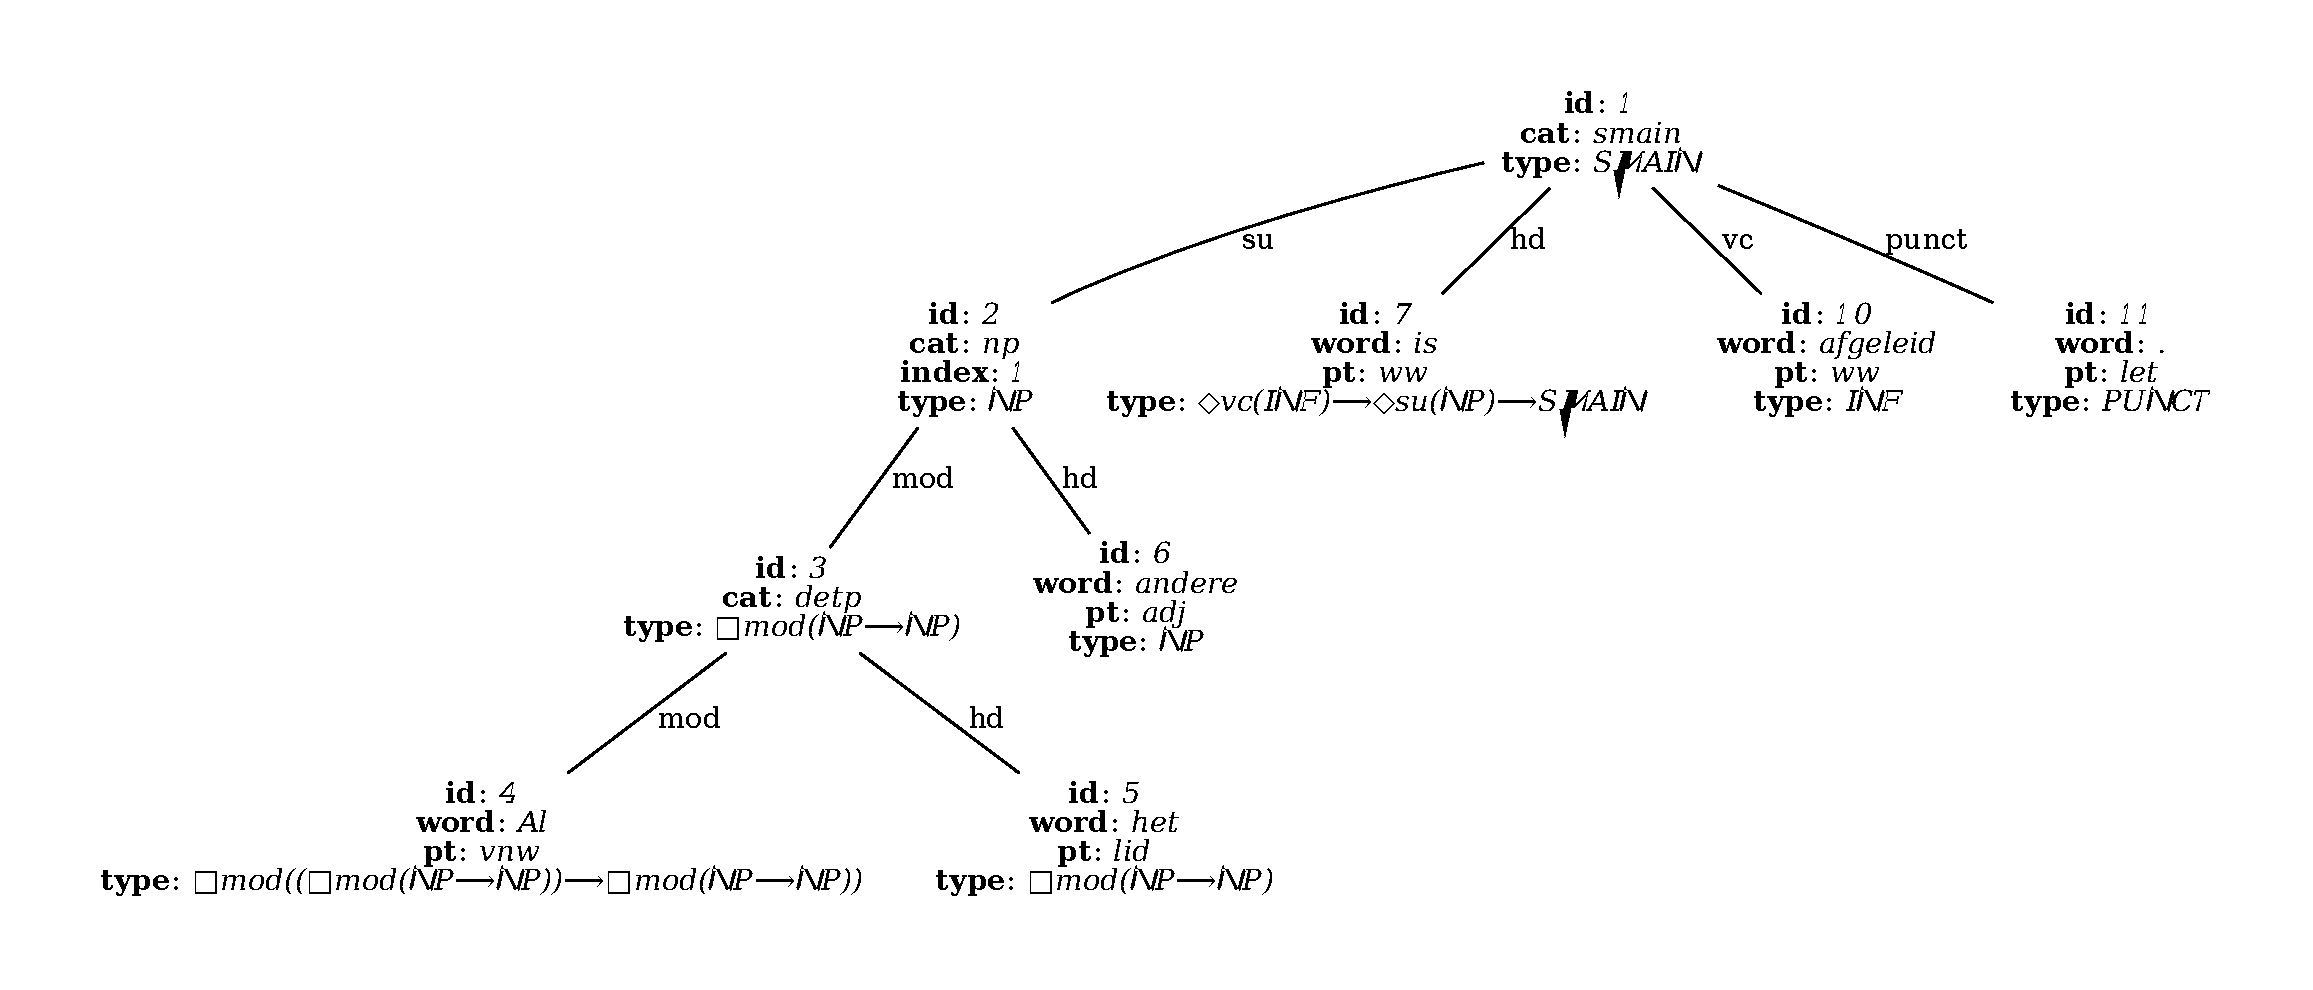
\includegraphics[width=1\textwidth, trim={1.5cm 1.5cm 1.5cm 1.5cm}]{./prebuilt/simple_extraction.pdf}
		\caption{Type-annotated sample.}
	\end{subfigure}\\[\midsep]
	\begin{subfigure}{1\textwidth}
		\resizebox{1\textwidth}{!}{
		\infer[\li E]
			{\con{7},\dbra{\con{10}}{vc},\dbra{\dbra{\dbra{\con{4}}{mod},\con{5}}{mod},\con{6}}{su}\vdash \smain}
			{
			\infer[\li E]
				{\con{7},\dbra{\con{10}}{vc}\vdash \ddia{su}\np\multimap \smain}
				{
				\infer[\Lex]
					{\con{7}: \ddia{vc}\ww\multimap \ddia{su}\np\multimap \smain}
					{}
				&
				\hspace{-5pt}
				\infer[\ddia{vc} I]
					{\dbra{\con{10}}{vc} \vdash \ddia{vc}\ww}
					{
					\infer[\Lex]
						{\con{10}: \ww}
						{}
					}
				}
			&
			\hspace{-105pt}
			\infer[\ddia{su} I]
				{\dbra{\dbra{\dbra{\con{4}}{mod},\con{5}}{mod},\con{6}}{su}\vdash \ddia{su}\np}
				{
				\infer[\li E]
					{\dbra{\dbra{\con{4}}{mod},\con{5}}{mod},\con{6}\vdash \np}
					{
					\infer[\dbox{mod} E]
						{\dbra{\dbra{\con{4}}{mod},\con{5}}{mod}\vdash \np\multimap \np}
						{
						\infer[\li E]
							{\dbra{\con{4}}{mod},\con{5}\vdash \dbox{mod}(\np\multimap \np)}
							{
							\infer[\dbox{mod} E]
								{\dbra{\con{4}}{mod}\vdash \dbox{mod}(\np\multimap \np)\multimap \dbox{mod}(\np\multimap \np)}
								{
								\infer[\Lex]
									{\con{4}: \dbox{mod}(\dbox{mod}(\np\multimap \np)\multimap \dbox{mod}(\np\multimap \np))}
									{}
								}
							&
							\infer[\Lex]
								{\con{5}: \dbox{mod}(\np\multimap \np)}
								{}
							}
						}
					&
					\hspace{-55pt}
					\infer[\Lex]
						{\con{6}: \np}
						{}
					}
				}
			}
		}
		\caption{Assigned proof (unprocessed).}
	\end{subfigure}\\[\midsep]
	\aethelcap
		{WR-P-E-I-0000041235.p.1.s.123(1)}
		{Al het andere is afgeleid.}
		{All the rest is derivative.}
		{\term{\con{7}~\ddiaintro{vc}\con{10}~\ddiaintro{su}(\dboxelim{mod}(\dboxelim{mod}\con{4}~\con{5})~\con{6})}}
	\caption{Proving a simple finite clause.}
	\label{figure:simple_extraction}
\end{figure}
%

\paragraph{Matrix Clauses}
A simple verbal domain consists of a single head, some complements and (possibly) some adjuncts  -- we'll arrange them in corresponding bins, with complements sorted by their obliqueness hierarchy and adjuncts sorted by their order of appearance in the sentence.
First, we'll call $\mathsf{prove}$ on each argument tree, passing its corresponding dependency edge and no type hint as arguments.
Each proof that does not correspond to an instance of the $\Ax$ rule, we will apply a diamond introduction over, to enforce the appropriate complement dependency (hypotheses are excluded due to \textit{already} being of the correct diamond type).
By isolating the result types of the proofs extracted this way, we can infer the type of the phrasal head.
We can thefore call $\mathsf{prove}$ on the head tree, passing no correspoding dependency edge, but type hinting it as the curried function from the sequentialized arguments to the top type.
In a dual fashion, we can call $\mathsf{prove}$ on each adjunct tree, type hinting it as the endomorphism of the top type, enclosed under a box of the corresponding dependency label.
With this and that, we now have proofs for each subtree underneath us -- what remains to be done is fusing these proofs together.
The way to go is simple: we need to first left fold the head's proof against the complements' proofs, and then apply the function composition of the ``unboxed'' adjuncts' proofs onto the result (unbox literally meaning using the box elimination rule to reveal the endomorphism enclosed within).
Let's reiterate this for clarity.
Each step of the initial fold will produce a ``shorter'' type, and, by the the time we run out of complements, the result's type will coincide with the top type.
Each unboxed adjunct will be a function from the top type to itself -- their n-ary function composition will then still be the of the same type, meaning it can be directly applied to our intermediate result.
At this point, we have each tree below exactly once (yay, linearity), and we have produced a proof of the type we were asked to (or the tree prescribed), meaning we're good to go.
Exceptionally to the above, nodes assigned the \textit{punct} tag are given a plain \smallgtype{punct} type that does not partake in the proof.

This simple setup already suffices to cover quite a lot of trees with simple applicative phenomena, including higher order modifiers like in the example of Figure~\ref{figure:simple_extraction}.
There, nodes 1, 2 and 10 obtains types $\smain[s]$, $\np[s]$ and $\ww[s]$ by simple translation, and 7 obtains the type $\ddia{vc}\ww[s]\li\ddia{su}\np[s]\li\smain[s]$, having 10 and 2 as complements (adorned with $\ddia{vc}$ and $\ddia{su}$ diamonds respectively) and 1 as the result.
Node 2 forces the type $\dbox{mod}(\np[s]\li\np[s])$ to node 3 (as an adjunct with the \textit{mod} label), in turn forcing the type $\dbox{mod}(\dbox{mod}(\np[s]\li\np[s])\li\dbox{mod}(\np[s]\li\np[s]))$ to node 4 for the exact same reason. 
Nodes 5 and 6 inherit the types of their mothers (3 and 2), having no complements.
Within each domain, heads apply to their arguments and adjuncts drop their boxes to apply to the result.

\begin{figure}
	\begin{subfigure}{1\textwidth}
		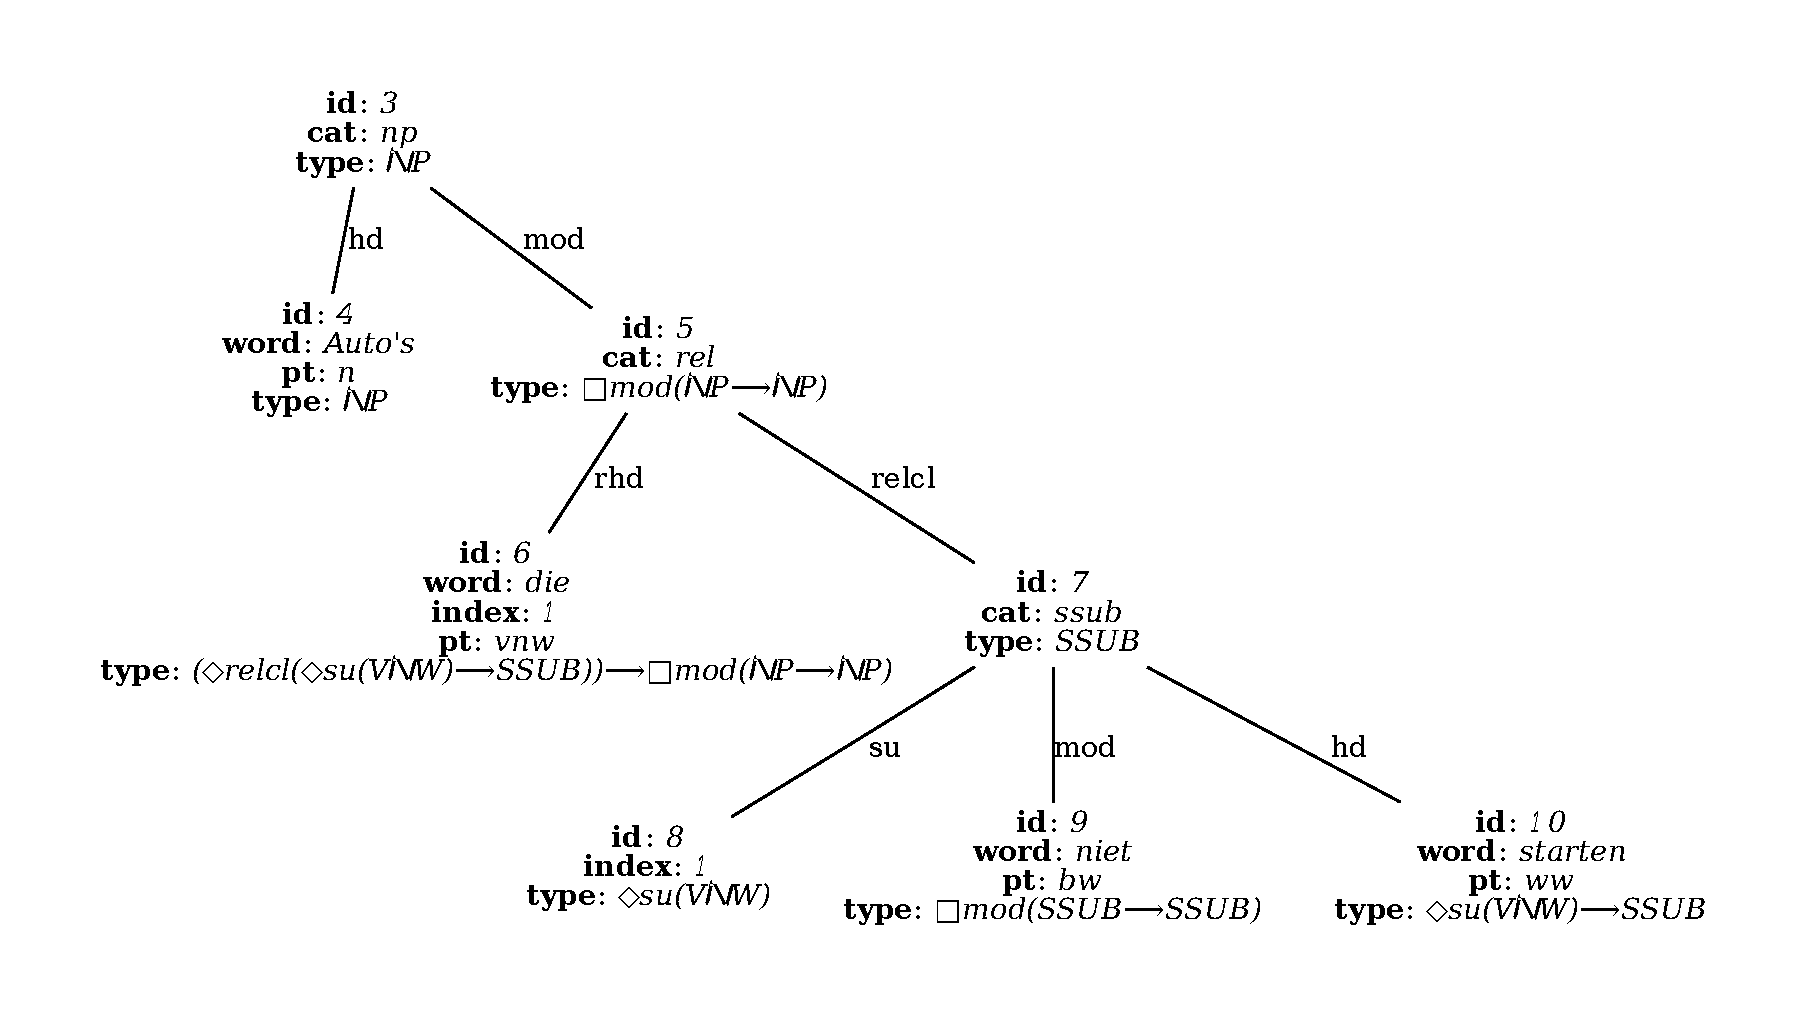
\includegraphics[width=1\textwidth, trim={1.5cm 1.5cm 1.5cm 1.5cm}]{./prebuilt/simple_abstraction.pdf}\\[\smallsep]
	\end{subfigure}\\[\midsep]
	\begin{subfigure}{1\textwidth}
		\resizebox{1\textwidth}{!}{
			\infer[\li E]{\dbra{\con{6},\dbra{\dbra{\con{9}}{mod},\con{10}}{relcl}}{mod},\con{4} \vdash \np}{
				\infer[\dbox{mod} E]{\dbra{\con{6},\dbra{\dbra{\con{9}}{mod},\con{10}}{relcl}}{mod} \vdash (\np\li\np)}{
					\infer[\li E]{\con{6},\dbra{\dbra{\con{9}}{mod},\con{10}}{relcl} \vdash \dbox{mod}(\np\li\np)}{
						\infer[\Lex]{\con{6}: \ddia{relcl}(\ddia{su}\vnw\li\ssub)\li\dbox{mod}(\np\li\np)}{}
						&
						\hspace{-30pt}
						\infer[\ddia{relcl} I]{\dbra{\dbra{\con{9}}{mod},\con{10}}{relcl} \vdash \ddia{relcl}(\ddia{su}\vnw\li\ssub)}{
							\infer[\li I]{\dbra{\con{9}}{mod},\con{10} \vdash \ddia{su}\vnw\li\ssub}{
								\infer[\li E]{\dbra{\con{9}}{mod},\con{10},\Var{8} \vdash \ssub}{
									\infer[\dbox{mod} E]{\dbra{\con{9}}{mod}}{
										\infer[\Lex]{\con{9} : \dbox{mod}(\ssub\li\ssub)}{}
									}
									&
									\infer[\li E]{\con{10},\Var{8} \vdash \ssub}{
										\infer[\Lex]{\con{10}: \ddia{su}\vnw\li\ssub}{}
										&
										\infer[\Ax]{\Var{8}: \ddia{su}\vnw}{}
									}
								}
							}
						}
					}
				}
				&
				\hspace{-50pt}
				\infer[\Lex]{\con{4}: \np}{}
			}
		}
	\end{subfigure}\\[\smallsep]
	\aethelcap
		{WS-U-E-A-0000000016.p.37.s.1(3)}
		{Auto's die niet starten.}
		{Cars that don't start.}
		{\term{\dboxelim{mod}(\con{6}~\ddiaintro{relcl}((\lam \Var{8}.\dboxelim{mod}\con{9}~(\con{10}~\Var{8}))))~\con{4}}}
	\caption{Abstracting over a relative clause gap.}
	\label{figure:simple_abstraction}
\end{figure}

\paragraph{Subordinate Clauses}
Now, if you have a sneaking suspicion that this looks oddly easy, you're right.
We have not yet made any attempt to cover cases of hypothetical reasoning triggered by relative clauses and wh-questions.
The hypotheses in such phenomena have already been established by the phantom nodes underlying them -- all we need to do is know when to withdraw them.
The criterion we'll follow applies to the proofs assigned to phrasal complements, and requires first that the phrasal head is indexed.
If that is the case, it draws out all variables within the proof investigated, and filters those of them whose node shares the same index as the head.
Variables caught are abstracted over before the diamond introduction rule is applied.
Figure~\ref{figure:simple_abstraction} presents a concrete example: node 6 carries index 1 and looks for its complement in node 7.
But node 7 contains $\Var{8}$, and node 8 has index 1 -- therefore, we must abstract the proof of node 7 over $\Var{8}$ before continuing with assigning it a diamond.

\begin{figure}
	\begin{subfigure}{1\textwidth}
		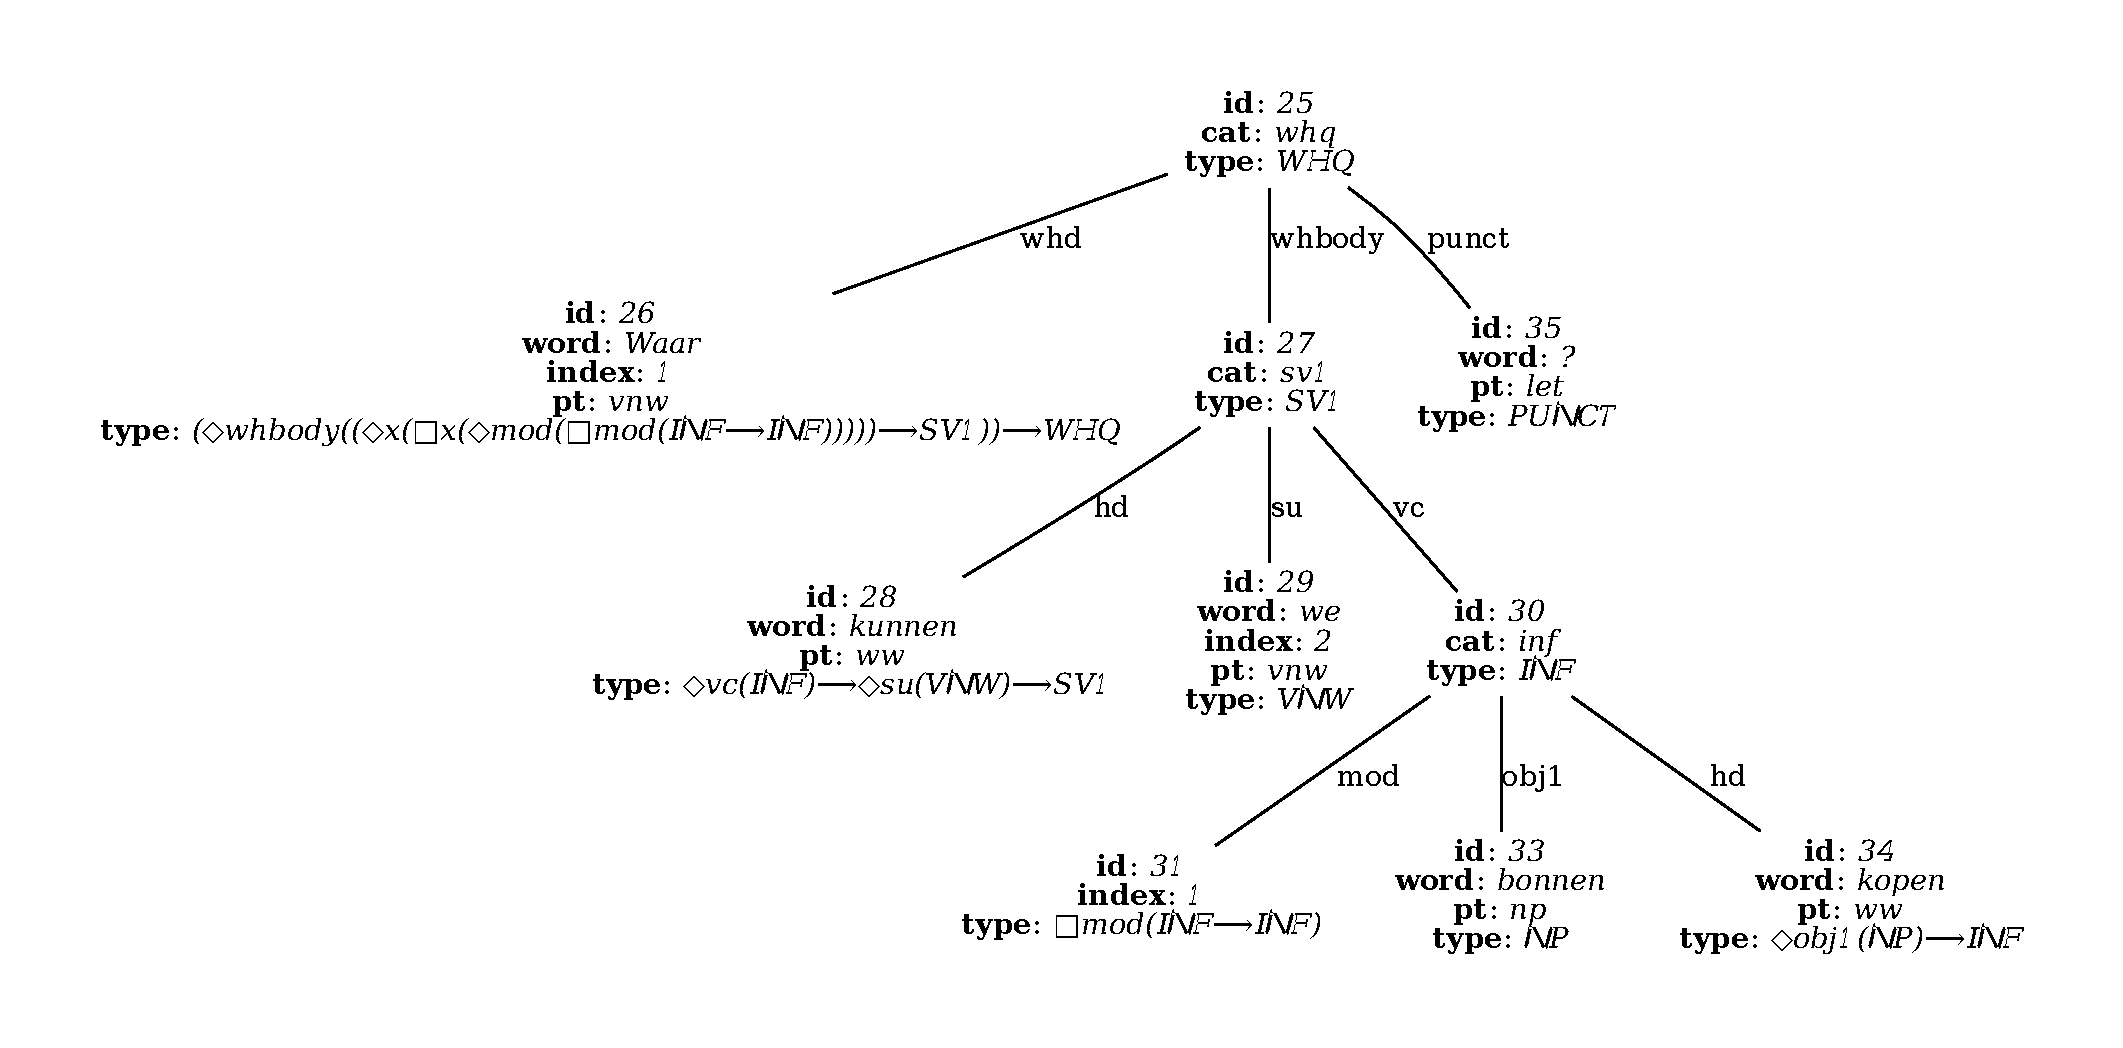
\includegraphics[width=1\textwidth, trim={1.5cm 1.5cm 1.5cm 1.5cm}]{./prebuilt/hard_abstraction.pdf}\\[\smallsep]
	\end{subfigure}\\[\midsep]
	\begin{subfigure}{1\textwidth}
		\resizebox{1\textwidth}{!}{
			\hspace{100pt}
			\infer[\li E]{\con{26},\dbra{\con{28},\dbra{\con{34},\dbra{\con{33}}{obj1}}{vc},\dbra{\con{29}}{su}}{whbody}\vdash\whq}{
				\infer[\Lex]{\con{26} : \ddia{whbody}(\dxdia{x}\dxbox{x}\ddia{mod}\dbox{mod}(\infp\li\infp)\li\svi)\li\whq}{}
				&
				\hspace{-350pt}
				\infer*[]{}{\infer*[]{}{
				\infer[\ddia{whbody} I]{\dbra{\con{28},\dbra{\con{34},\dbra{\con{33}}{obj1}}{vc},\dbra{\con{29}}{su}}{whbody} \vdash \ddia{whbody}(\dxdia{x}\dxbox{x}\ddia{mod}\dbox{mod}(\infp\li\infp)\li\svi)}{
					\infer[\li I]{\con{28},\dbra{\con{34},\dbra{\con{33}}{obj1}}{vc},\dbra{\con{29}}{su} \vdash \dxdia{x}\dxbox{x}\ddia{mod}\dbox{mod}(\infp\li\infp)\li\svi}{
						\infer[\dxdia{x} E]{\con{28},\dbra{\con{34},\dbra{\con{33}}{obj1}}{vc},\Var{31}'',\dbra{\con{29}}{su} \vdash\svi}
						{
							\infer[\Extraction]{\con{28},\dbra{\con{34},\dbra{\con{33}}{obj1}}{vc},\dbra{\Var{31}'}{x},\dbra{\con{29}}{su} \vdash\svi}{
								\infer[\li E]{\con{28},\dbra{\dbra{\Var{31}'}{x},\con{34},\dbra{\con{33}}{obj1}}{vc},\dbra{\con{29}}{su} \vdash\svi}{
									\infer[\li E]{\con{28},\dbra{\dbra{\Var{31}'}{x},\con{34},\dbra{\con{33}}{obj1}}{vc} \vdash \ddia{su}\vnw\li\svi}{
										\infer[\Lex]{\con{28}: \ddia{vc}\infp\li\ddia{su}\vnw\li\svi}{}
										&
										\hspace{-160pt}
										\infer[\ddia{vc} I]{\dbra{\dbra{\Var{31}'}{x},\con{34},\dbra{\con{33}}{obj1}}{vc} \vdash \ddia{vc}\infp}{
											\infer[\li E]{\dbra{\Var{31}'}{x},\con{34},\dbra{\con{33}}{obj1} \vdash \infp}{
												\infer[\ddia{mod} E]{\dbra{\Var{31}'}{x} \vdash \infp\li\infp}{
													\infer[\dbox{mod} E]{\dbra{\Var{31}}{mod} \vdash \infp\li\infp}{
														\infer[\Ax]{\Var{31}: \dbox{mod}(\infp\li\infp)}{}
													}
													&
													\infer[\dxbox{x} E]{\dbra{\Var{31}'}{x} \vdash \ddia{mod}\dbox{mod}(\infp\li\infp)}{
														\infer[\Ax]{\Var{31}' : \dxbox{mod}\ddia{mod}\dbox{mod}(\infp\li\infp)}{}
													}
												}
												&
												\infer[\li E]{\con{34},\dbra{\con{33}}{obj1} \vdash \infp}{
													\infer[\Lex]{\con{34}: \ddia{obj1}\np\li\infp}{}
													&
													\infer[\ddia{obj1} I]{\dbra{\con{33}}{obj1} \vdash \ddia{obj1}\np}{
														\infer[\Lex]{\con{33}: \np}{}
													}
												}
											}
										}
									}
									&
									\hspace{-100pt}
									\infer[\ddia{su} I]{\dbra{\con{29}} \vdash \ddia{su}\vnw}{
										\infer[\Lex]{\con{29}: \vnw}{}
									}
								}
							}
							&
							\hspace{-75pt}
							\infer[\Ax]{\Var{31}'' : \dxdia{x}\dxbox{x}\ddia{mod}\dbox{mod}(\infp\li\infp))}{}
						}
					}
				}
			}
			}
			}
		}
	\end{subfigure}\\[\smallsep]
	\aethelcap
		{WR-P-E-I-0000039352.p.3.s.7(25)}
		{Waar kunnen we bonnen kopen?}
		{Where can we buy beans?}
		{\smaller
		\term{\con{26}~
			\ddiaintro{whbody}(\lam \Var{31}''.
			\caseof
				{\ddiaelim{x}\Var{31}''}
				{\Var{31}'}
				{(\con{28}~\ddiaintro{vc}
					(\caseof
						{\ddiaelim{mod}\dboxelim{x}\Var{31}'}
						{\Var{31}}
						{(\dboxelim{mod}\Var{31}~(\con{34}~\ddiaintro{obj1}\con{33}))})
				~\ddiaintro{su}\con{29})
				)}
			)
		}}
	\caption{Abstracting over a nested adjunct.}
	\label{figure:hard_abstraction}
\end{figure}


\paragraph{Horrors from the Deep}
But can we really be certain that the abstraction is indeed possible?
Recalling once more our discussion from Section~\ref{subsubsection:sreason_dep}%
	\footnote{The variable may be free, but it could lie inaccessible behind structural brackets -- don't mention it.},
there's a very real risk we might end up getting locked out of our hypotheses when these are adjuncts, nested deeply, or both.
In the first case, we need to reproduce our strategy from Figure~\ref{figure:higher_order_dep}.
To do so, we need the tiniest of adaptations to our ``unbox-and-apply'' scheme from earlier on -- when the adjunct that was unboxed happens to be a variable, we will immediately follow through with a diamond elimination.
This way, when the time comes for us to be abstract over the reclusive adjunct (and the time will come, since our proofs must be linear), it will already have been liberated of its structural brackets.
In the second case, we are in trouble. 
We need to employ the structural licensing pair $\dxdia{x}\dxbox{x}$, as in Figure~\ref{figure:higher_order_nested_dep}, but there is no way for the proof assignment to have been correct preemptively: we would have needed to know that the variable is nested before ever getting to actually build its nesting context.
To solve this chicken and egg problem, we need to allow ourselves an erroneous assignment, and then travel back in time to retroactively correct it.
No big deal: going back in time means simply applying the substitution meta-pattern $\vari^{\smallgtype{a}} \mapsto \dboxelim{x}(\vari^{\dxbox{x}\smallgtype{a}})$.
In non-obscure, this translates to traversing the proof, finding the problematic hypothesis and replacing it with an $\dep{x}$-marked (i.e. extractable) equivalent.
Reconstructing the proof is not sufficient though -- we also need to perform all the $\Extraction$ rules necessary for the $\dep{x}$-marked structure to always appear at the structural onion's outermost layer, as well as substitute it for its logical diamond counterpart.
At that point, we are at long last able to abstract over the hypothesis.

The conventions described serve also to impose a canonical placement for the diamond elimination pattern.
In combination with our carefully planned formulation of the $\Extraction$ rule from Section~\ref{subsubsection:sreason_dep}%
	\footnote{As strictly localized and with shallow context -- anytime.},
we have effectively relieved the burden of proof equivalence checking: diamond eliminations are to be performed as soon as possible and structural extractions as late as possible (but no later) -- i.e. we will avoid perpetuating temporary structures unless they have a purpose.
To see this in action, let's have a look at the example of Figure~\ref{figure:hard_abstraction}.
There, node 31 is originally assigned $\Var{31} : \dbox{mod}(\infp[s]\li\infp[s])$.
Upon unboxing it for application, we realize it's a hypothetical adjunct, therefore we follow through with a diamond elimination to $\Var{31}' : \ddia{mod}\dbox{mod}(\infp[s]\li\infp[s])$ to lose the \dep{mod} brackets.
Further down the line, we attempt to abstract over $\Var{31}'$, only to find it trapped in a $\dep{vc}$ bracket.
To facilitate the emancipation of the hypothesis, we perform the meta-syntactic substitution $\Var{31}' \mapsto \dboxelim{x}\Var{31}'$, where the new $\Var{31}'$ is of type $\dxbox{x}\ddia{mod}\dbox{mod}(\infp[s]\li\infp[s])$.
Empowered by its black box, the variable breaks free of its chains with the $\Extraction$ rule, and gets diamond eliminated to $\Var{31}'' : \dxdia{x}\dxbox{x}\ddia{mod}\dbox{mod}(\infp[s]\li\infp[s])$.
The latter is bracketless and exactly where we want it -- we can finally perform the abstraction.

\paragraph{Nominal Domain}
The situation is not much different in the nominal domain, except for a change in the order we do things in.
%Our separation of noun and noun-phrase modifiers in two layers will now save us the trouble of having to resolve any  conflicts between determiners and modifiers.
First, we must call $\mathsf{prove}$ on the head; unlike before, it receives no type hint, as we do not expect it to come out as a functor.
Next, we requisit a proof for the determiner, hinted as a function from the head's type to the top type (with a complementary box on top, of course).
Last, we ask for a proof for each adjunct, again as the boxed endomorphism of the result.
Same as before, we take the function composition of all adjuncts; determiner first, since it's the one responsible for raising the noun to a noun phrase, followed by the garden variety modifiers in order of appearance.
At this point, we must thank our past selves for the separation of noun and noun-phrase modifiers in two different tree layers, as this has saved us the trouble of having to scratch our head contemplating how to organize adjuncts.

\paragraph{Conjunctions}
We are almost there.
The last bit remaining is unfortunately also the hardest one: conjunctions.
Conjunctions are the infernal harbinger of torment and despair.
Their ability to use linguistic material more than once challenges the linearity of our type system.
To overcome their dark influence, we'll need to resort to arcane conjurations from the ancient texts (summarized for your convenience in Chapter~\ref{chapter:Introduction}).

A few conjunctions are actually innocuous, i.e. when the tree inspected consists of a single coordinator and a sequence of conjuncts.
Porting our intuitions on coordinator type assignments from Section~\ref{subsubsection:intricacies}%
	\footnote{Coordinators are polymorphic types binding pairs of the same type into a conjoined pair -- no problem.}%
, we obtain the recipe $\ddia{cnj}\chi\li\ddia{cnj}\chi\li\chi$, where $\chi$ is to range over types.
In the vanilla case, we may simply call $\mathsf{prove}$ on each conjunct independently, hinting each as the top type (which, if not hinted, will be the translation of the syntactic category labels' majority consensus).
Then, we may move on to the coordinator, which is hinted as a function from the ($\ddia{cnj}$-marked) conjuncts' types to the top type.
Having used the same type hint amounts to a coercion that ensures that the parts and the whole are of the same type -- in other words, we are faithful to our polymorphic recipe.
A minor divergence is that our coordinator type is slightly more general than originally prescribed, being a variadic function rather than a binary one, since Lassy conjunctions are flat trees rather than hierarchical ones (punctuations carrying no annotations by default).

\begin{figure}
	\begin{subfigure}{1\textwidth}
		\includegraphics[width=1\textwidth, trim={1.5cm 1.5cm 1.5cm 1.5cm}]{./prebuilt/subj_ellipsis.pdf}\\[\smallsep]
	\end{subfigure}\\[\midsep]
	\begin{subfigure}{1\textwidth}
		\resizebox{1\textwidth}{!}{
			\infer[\li E]{\con{5},\dbra{\con{4}}{cnj},\dbra{\con{8}}{cnj},\dbra{\con{3}}{su} \vdash \smain}{
				\infer[\li E]{\con{5},\dbra{\con{4}}{cnj},\dbra{\con{8}}{cnj} \vdash \ddia{su}\np\li\smain}{
					\infer[\li E]{\con{5},\dbra{\con{4}}{cnj} \vdash \ddia{cnj}\chi\li\chi}{
						\infer[\Lex]{\con{5}: \ddia{cnj}\chi\li\ddia{cnj}\chi\li\chi}{}
						&
						\hspace{-10pt}
						\infer[\ddia{cnj} I]{\dbra{\con{4}}{cnj} \vdash \ddia{cnj}\chi}{
							\infer[\li I]{\con{4} \vdash \ddia{su}\np\li\smain}{
								\infer[\li E]{\con{4},\Var{9} \vdash \smain}{
									\infer[\Lex]{\con{4}: \ddia{su}\np\li\smain}{}
									&
									\infer[\Ax]{\Var{9}: \ddia{su}\np}{}
								}
							}
						}
					}
					&
%					\hspace{-170pt}
					\infer[\ddia{cnj} I]{\dbra{\con{8}}{cnj} \vdash \ddia{cnj}\chi}{
						\infer[\li I]{\con{8} \vdash \ddia{su}\np\li\smain}{
							\infer[\li E]{\con{8},\Var{9} \vdash \smain}{
								\infer[\Lex]{\con{8}: \ddia{su}\np\li\smain}{}
								&
								\infer[\Ax]{\Var{7}: \ddia{su}\np}{}
							}
						}
					}
				}
				&
%				\hspace{-100pt}
				\infer[\ddia{su} I]{\dbra{\con{3}}{su} \vdash \ddia{su}\np}{
					\infer[\Lex]{\con{3} : \np}{}
				}
			}
		}	
	\end{subfigure}\\[\smallsep]
	\aethelcap
		{wiki-6984.p.6.s.2(1)}
		{Onafhankelijkheid moet en kan.}
		{Independence must and can (happen).}
		{\term{\con{5}~\ddiaintro{cnj}(\lam \Var{9}.\con{4}~\Var{9})~\ddiaintro{cnj}(\lam\Var{7}.\con{8}~\Var{7})~\ddiaintro{su}\con{3}}}
	\caption{Proving a subject ellipsis.}
	\label{figure:subj_elipsis}
\end{figure}

Unlike their well-behaved kindred, elliptical conjunctions require special treatment.
Lassy rightly prefers pushing conjunctions to the topmost phrasal level.
The subject ellipsis of Figure~\ref{figure:subj_elipsis}, for instance, is not annotated as the conjunction of two heads applied to a single noun phrase, but rather as the conjunction of two sentences sharing the same subject (the material subject has been elevated to the same level as the conjuncts thanks to our earlier transformation).
We'll gladly follow along.
Same as before, we will first seek a proof for each conjunct, but now also any non-conjunct siblings. % marked with a complement dependency.
Conjuncts containing any variables whose nodes are coindexed with the non-conjunct siblings (the latter necessarily being material counterparts of conjunct-internal phantoms) will be abstracted over these variables, before being marked by the $\ddia{cnj} I$ rule.
In the running example,  conjunct 2 contains the phantom subject 9 and conjunct 6 the phantom subject 7, both coindexed with material node 3.
The proofs of 2 and 6 will therefore be abstracted over their subject variables, and the instantiation of the type variable $\chi$ will in this case be $\ddia{su}\np[s]\li\smain[s]$ (intentionally left implicit in the Figure for space economy).
The proof we get back is coincidentally an $\eta$-expanded version of the heads' conjunction.

What if the elided item is not a complement, though?
Not much changes, really: we must still look for hypotheses ``shared'' between adjuncts and materially present in the current conjunction branch.
The difference is that withdrawing them this time around yields proofs of higher-order types.
To see this in practice, let's consider the example of Figure~\ref{figure:vp_ellipsis}%
	\footnote{Give it up for our first ever landscape proof!}.
Conjuncts 14 and 24 contain phantom 33 and 25 respectively, both standing in for a matrix head, implementing a function of the same type, and coindexed with the same material node 19.
The abstraction will result in type variable $\chi$ being instantiated as the second order type $(\ddia{vc}\ww\li\ddia{su}\np\li\smain)\li\smain$, in turn producing a third order type hint for the coordinator... oof.

Complicated as it might be, this type should not be alien to you, diligent reader.
Let's flip things around and focus on what we have instead of what we miss.
The dual view of having two sentences missing their head is that we have two pairs of floating constituents, pair one made of the modally marked proofs of nodes 15 and 22, and pair two made of the proofs of nodes 26 and 31.
If we were to allow products in our type calculus, we could encode each pair as an item of type $\ddia{su}\np[s]\otimes\ddia{vc}\ww$, and use this to instantiate the polymorphic type.
By type raising, we could alternatively use them to derive corresponding proofs of type $((\ddia{su}\np[s]\otimes\ddia{vc}\ww)\li\smallgtype{a})\li\smallgtype{a}$, for any $\smallgtype{a}$ of our liking.
By currying, we would end up with sequentialized versions of type $(\ddia{su}\np[s]\li\ddia{vc}\ww\li\smallgtype{a})\li\smallgtype{a}$.
Ring a bell yet?
Using $\smain[s]$ in place of $\smallgtype{a}$, we end up exactly where we started.%
	\footnote{If this made little sense, you should actually read the introduction instead of relying on footnote clues.
	Also I take ``diligent'' back.}
Now, toying around with raised types is by no means ideal, as it reinforces the propensity of coordinators to become very long and complex.
On the other hand, it absolves us from having to incorporate an explicit product and protects us from the headaches it comes with (like proof equivalence under product elimination, type equivalence under different branchings, more latex symbols to render in console pretty printing, etc., just to name a few).
On the less cynical side, it also has the merit of permitting more flexible semantic interpretations for the user to be.
Conjoining a series of arguments and feeding the result to the predicate means that the semantic interpretation of the coordinator would be inescapably bound to a local scope.
Conjoining a series of $\lambda$ abstractions and applying the result to the shared predicate grants the coordinator access to the full context of the conjunction, opening the door to a future semantic interpretation that can duplicate and distribute meaning if and as desired.

\begin{sidewaysfigure}
	\begin{subfigure}{1\textwidth}
		\centering
		{\includegraphics[width=0.85\textheight, trim={1.5cm 1.5cm 1.5cm 1.5cm}]{./prebuilt/hd_ellipsis.pdf}}
	\end{subfigure}\\[\midsep]
	\begin{subfigure}{1\textwidth}
		\resizebox{1\textwidth}{!}{
			\infer[\li E]{\con{23},\dbra{\dbra{\con{22}}{vc},\dbra{\dbra{\con{16}}{mod},\dbra{\con{17}}{mod},\con{18}}{su}}{cnj},\dbra{\dbra{\con{31}}{vc},\dbra{\dbra{\con{27}}{det},\con{28}}{su}}{cnj},\con{19} \vdash \smain}{
				\infer[\li E]{\con{23},\dbra{\dbra{\con{22}}{vc},\dbra{\dbra{\con{16}}{mod},\dbra{\con{17}}{mod},\con{18}}{su}}{cnj},\dbra{\dbra{\con{31}}{vc},\dbra{\dbra{\con{27}}{det},\con{28}}{su}}{cnj} \vdash \chi}{
					\infer[\li E]{\con{23},\dbra{\dbra{\con{22}}{vc},\dbra{\dbra{\con{16}}{mod},\dbra{\con{17}}{mod},\con{18}}{su}}{cnj} \vdash \ddia{cnj}\chi\li\chi }{
						\infer[\Lex]{\con{23} : \ddia{cnj}\chi\li\ddia{cnj}\chi\li\chi}{}
						&
						\infer[\ddia{cnj}I]{\dbra{\dbra{\con{22}}{vc},\dbra{\dbra{\con{16}}{mod},\dbra{\con{17}}{mod},\con{18}}{su}}{cnj} \vdash \ddia{cnj}\chi}{
							\infer[\li I]{\dbra{\con{22}}{vc},\dbra{\dbra{\con{16}}{mod},\dbra{\con{17}}{mod},\con{18}}{su} \vdash \chi}{
								\infer*{\Var{33},\dbra{\con{22}}{vc},\dbra{\dbra{\con{16}}{mod},\dbra{\con{17}}{mod},\con{18}}{su} \vdash \smain}{
								}
%									\infer[\li E]{\Var{33},\dbra{\con{22}}{vc} \vdash \ddia{su}\np\li\smain}{
%										\infer[\Ax]{\Var{33}: \ddia{vc}\ww\li\ddia{su}\np\li\smain}{}
%										&
%										\infer[\ddia{vc}I]{\dbra{\con{22}}{vc} \vdash \ddia{vc}\ww}{
%											\infer[\Lex]{\con{22} : \ww}{}
%										}
%									}
%									&
%									\infer[\ddia{su}I]{\dbra{\dbra{\con{16}}{mod},\dbra{\con{17}}{mod},\con{18}}{su} \vdash \ddia{su}\np}{
%										\infer*{\dbra{\con{16}}{mod},\dbra{\con{17}}{mod},\con{18}\vdash \np}{}
%									}
%								}
							}
						}
					}
					&
					\infer[\ddia{cnj}I]{\dbra{\dbra{\con{31}}{vc},\dbra{\dbra{\con{27}}{det},\con{28}}{su}}{cnj} \vdash \ddia{cnj}\chi}{
						\infer[\li I]{\dbra{\con{31}}{vc},\dbra{\dbra{\con{27}}{det},\con{28}}{su} \vdash \chi}{
							\infer*{\Var{25},\dbra{\con{31}}{vc},\dbra{\dbra{\con{27}}{det},\con{28}}{su} \vdash \smain}{
							}
%								\infer[\li E]{\Var{25},\dbra{\con{31}}{vc} \vdash \ddia{su}\np\li\smain}{
%									\infer[\Ax]{\Var{25}: \ddia{vc}\ww\li\ddia{su}\np\li\smain}{}
%									&
%									\infer[\ddia{vc}I]{\dbra{\con{31}}{vc} \vdash \ddia{vc}\ww}{
%										\infer[\Lex]{\con{31} : \ww}{}
%									}
%								}
%								&
%								\infer[\ddia{su}I]{\dbra{\dbra{\con{27}}{det},\con{28}}{su}\vdash\ddia{su}\np}{
%									\infer*{\dbra{\con{27}}{det},\con{28}\vdash\np}{}
%								}
%							}
						}
					}
				}
				&
				\infer[\Lex]{\con{19}: \ddia{vc}\ww\li\ddia{su}\np\li\smain}{}
			}
		}
	\end{subfigure}\\[\smallsep]
	\aethelcap
		{WR-P-E-I-0000015007.p.1.s.146(13)}
		{Vele Palestijnse huizen werden opgeblazen en hun bewoners vermoord.}
		{Many Palestinian houses were destroyed and their residents murdered.}
		{\term{\con{23}~
			\ddiaintro{cnj}(\lam \Var{33}.\Var{33}~\ddiaintro{vc}\con{22}~\ddiaintro{su}(\dboxelim{mod}\con{16}~(\dboxelim{mod}\con{17}~\con{18}))
			~\ddiaintro{cnj}(\lam \Var{25}.\Var{25}~\ddiaintro{vc}\con{31}~\ddiaintro{su}(\dboxelim{det}\con{27}~\con{28}))
			~\con{19}}}
	\caption{Proving a verb phrase ellipsis.}
	\label{figure:vp_ellipsis}
\end{sidewaysfigure}

More generally, the proof of each conjunct will contain a mixture of constants and variables, the latter being any combination of heads, complements and adjuncts.
All ``shared'' variables will be abstracted over.
To maintain the homogeneousness of functors regardless of the context they appear in, the order of abstraction is reverse to the obliqueness hierarchy we have used so far.
Head- and adjunct- functors, falling outside the hierarchy, will have priority over complements, appearing as the first argument of the higher-order types they help form.
Any secondary coordinator appearing within the same conjunction (its dependency now labeled \textit{cor}, due to our earlier transformation), will be the first argument to be consumed by the main coordinator (the two are thus modeled as a derived and discontinuous coordinator phrase).

\subsubsection{Post-Processing}
The proofs we get back don't need to be type-checked: the extraction has already taken care of that for us.
From the type-correctness perspective, all we need to do is assert their linearity in terms of both variables and constants, i.e. make sure that all words of the input sample were used (exactly once each), and ditto for variables, except they must also be bound (in the off chance a phantom node was never abstracted over).
For the sake of uniformity, all proofs obtained are $\beta$ and $\eta$ reduced.
From the representation perspective, our proofs are still overly attached to their Lassy roots.
Constants and variables are named according to their node origins, which will no longer make any sense after the tree has been discarded.
We therefore rename constants according to their order of appearance in the sentence, and variables by enumeration, following a left-first depth-first traversal of the proof tree (preferrable to de Bruijn indexing for human legibility).
To allow the incorporation of extra-theoretical information, proofs are repackaged into a $\mathsf{Sample}$ record containing fields $\mathsf{proof}$, $\mathsf{lexical\_phrases}$, $\mathsf{name}$ and $\mathsf{subset}$.
The first field is self-explanatory.
The second field contains a variadic tuple of lexical phrases, each element being itself a variadic container of lexical items, given a single type assignment as a whole.
Each lexical item contains node attributes from the original Lassy annotation, like $\mathsf{word}$, $\mathsf{pos}$, $\mathsf{pt}$ and $\mathsf{lemma}$.
This organization is in line with the more liberal type lexicon demanded by multiword units, and allows us to preserve lexical information that would be lost if we were to simply just squeeze them into a single ``word''.
Multiwords aside, it faithfully presents a sentence together with its punctuation marks, despite them not (usually) appearing in the compositional analysis.
Finally, it disassociates proofs from the concrete lexical constants justifying them, allowing us to easily compare, filter and aggregate proofs detached from the sentences they were assigned to.
The third field simply associates the sample to its Lassy identifier, whereas the fourth field suggests a standard train/dev/test split for machine learning applications.
The collection of extracted proofs we will call \AE thel, for Automatically Extracted Theorems from Lassy, thus resolving the mystery of this section's cryptic name for those that made it this far.

% problems
% atomic types? 
%	n vs np, ww vs ppart vs inf vs ppres
% shared vs distributed adjuncts?

% how-to?

\subsection{Analysis}
\subsubsection{Quantitative Snoozefest}
We are done with proving; time to get to counting.
But first, a disclaimer.
The numbers reported below have been relatively stable, but may well get to differ in between the time I write these words and the time you get to read them.
They are correct in my subjective frame of reference (version), namely $\mathtt{1.0.0a4}$. 

\paragraph{From Lassy to \AE thel}
From the 65\,200 trees of Lassy Small, we discard 2\,607 for being a single word or punctuation mark.
The remaining 62\,593 are pruned into 69\,613 discourse-free cuttings (1.11 cuttings per source tree, on average).
From these, the extraction algorithm produces 68\,782 theorems, bringing its (processed) corpus coverage to 98.81\%.
A random 80/10/10 split is applied to the source Lassy samples, which translates into 56\,895  train, 6\,119 (8.8\%) dev and 5\,768 (8.3\%) test \AE thel samples (81.7/8.8/8.3).
Performing the split on Lassy rather than directly on \AE thel ensures consistency between different revisions, and asserts that any sample overlap from subtree duplications during pruning will be contained within the same subset, keeping cross-contamination to a minimum.

%Ill-formed trees are almost always to blame for a failed extraction; most failures are either due to conjunctions without a coordinator, or because of linearity breaches (free variables that cannot be justified by an existing proof pattern).

To quantititatively measure the impact of the preprocessing transformations (i.e. see how close the derived dataset is to the original), we first examine how many of Lassy's samples are proven unaltered.
In line with our observations on discourse level annotations from earlier, we find that 48\,074 (76.80\%) of Lassy samples can be uniquely mapped to an \AE thel proof.
Counting the number of samples enumerating a certain number of words, we arrive at the graph of Figure~\ref{figure:count_lens}.
Surprising noone, the graph reveals that both the original and the derived corpus exhibit a right-skewed distribution of sample lengths, the latter being a left-shifted version of the former.
Concretely, Lassy has a mode of 13 and a median of 16.7 (ignoring the one-word sentences, for fairness), whereas \AE thel has a mode of 10 and a median of 15.
The difference between them is not that striking and really only affects their left tails and centers; in fact, the two distributions go almost hand in hand towards their right tails.
Practically, we lose a small proportion of originally long and medium-sized samples, and the broken parts accumulate into a bulk of short and really short samples (hence the outlier peak at 2).
Not bad, considering.

\begin{figure}
	\centering
	\begin{tikzpicture}
	\begin{axis}[
%	    title={Sample Counts by Length},
	    xlabel={Sample Length},
	    ylabel={Sample Count},
	    xmin=1, xmax=48,
%	    ymin=-0, ymax=1,
%	    xtick={1,10,100,1000,10000, 100000},
	    legend pos=north west,
	    ymajorgrids=true,
		minor y tick num=1,
	    yminorgrids=true,
	    xmajorgrids=true,
	    xminorgrids=true,
	    minor x tick num=1,
	    axis line style={draw=none},
	    tick style={draw=none},
%	    width=0.95\textwidth,
        legend pos=north east,
	]
	% lens
	\addplot[black, dashed, thick,smooth]
		table[
	    mark=none,
	    x index=0,
	    y index=1,
	    col sep=comma,
	    ] {data/aethel_lens.dat};
	\addlegendentry{\AE Thel}
	    
 	\addplot[black, smooth]
		table[
	    mark=none,
	    x index=0,
	    y index=1,
	    col sep=comma,
	    ] {data/lassy_lens.dat};
	\addlegendentry{Lassy}
	 \end{axis}
	\end{tikzpicture}
	\caption{Sample counts by length.}
	\label{figure:count_lens}
\end{figure}


\paragraph{Theorems}
To quantify the proof-theoretic diversity of the 68\,782 extracted samples, we abstract away from the sentences and end up with a total of 55\,052 unique theorems.
Figure~\ref{figure:proof_assignments} groups and displays them according to how common they are, i.e. how many times we see the same theorem associated to a different sentence.
Evidently, the vast majority of unique theorems (52\,665 or 95.7\%) occur but a single time within the dataset (i.e. they are assigned to a single sample), with logarithmically\textsubscript{10} fewer theorems being assigned to exponentially\textsubscript{2} more sentences, making \AE thel a rich and intricate resource.

\begin{figure}
	\centering
	\begin{tikzpicture}
	\begin{loglogaxis}[
	    xlabel={Times Theorems were Assigned},
	    ylabel={Number of Theorems},
	    legend pos=north west,
	    ymin=1,
	    xmin=0.9,
	    log basis x=2,
	    ybar interval=1,
	    nodes near coords, 
   	    every node near coord/.append style={xshift=10pt, font=\footnotesize},
		nodes near coords style={/pgf/number format/.cd, 1000 sep={\,},},
		log origin y=infty,
		point meta=rawy,
	]
	
	\addplot[black
	,postaction={pattern=north east lines}]
%	[black, const plot, dashdotdotted, thick]
		table[
	    x index=0,
	    y index=1,
	    col sep=comma,
	    ] {data/proof_counts.dat};
	\end{loglogaxis}
	\end{tikzpicture}
	\caption{Proof sparsity in \AE thel.}
	\label{figure:proof_assignments}
\end{figure}

\paragraph{Proof Ambiguity}
We've already made peace with the fact that our type logic is syntactically underspecified and prone to overgeneration.
But a side-effect of this concession is our inability to tell well- and ill- founded ambiguities apart, i.e. we have no means of knowing whether a second proof derivable from the exact same proof frame (sequence of type assignments) is a clear-cut error or indeed a linguistically plausible alternative reading.
Lassy itself only provides the derivation of one single reading (and it is not our place to ask which reading that is).
We can use this to our advantage to try and estimate the \textit{real} derivational ambiguity of \AE thel, by first isolating the proof frame of each sample (taking the type sequence independent of the sentence it was assigned to), and then counting the amount of unique proofs derived from each frame.%
	\footnote{Note that we are gathering \textit{just} the sequence of types assigned to a sample and \textit{not} the proof's antecedent, since the modal bracketing structure already disambiguates the proof assignment.}
In total, there's 56\,050 proof frames, but 53\,730 of those occur only once, thus being of little use to our purposes (since each will unavoidably be mapped to a single proof).
Of the remaining 2\,320, 2\,259 (97.4\%) are mapped to one unique proof, whereas 61 (2.6\%) may derive one of two unique proofs.
Using this as a guideline, we find 472 potentially ambiguous samples in the entirety of \AE thel (a measly 0.7\%), their frames being among the 61 suspects.
Manual inspection reveals most of them to really be ambiguous (e.g. the proof assigned prescribes one of two possible modifier attachments), 
although in some cases the alternative reading is linguistically ruled out on the basis of selectional restrictions.
Repeating the above after first casting the proof and type assignments to \NLP{} (dropping any dependency information via a stripping morphism), we end up with 55\,096 unique frames for 54\,065 unique proofs, with 2\,524 frames occurring more than once.
Of these, 2\,405 are behind 1 unique proof, 112 behind 2, 6 behind 3, and 1 is behind 5.
Potentially ambiguous samples are now doubled (909 or 1.7\% of the total), and ambiguities are more commonly artificial; would-be alternative readings for the newly ambiguous samples are usually ruled out by morphosyntactic constraints invisible to the theory.

What are all these boring numbers trying to tell us?
Well, two things.
First, that using an undirectional logical core doesn't really estrange the grammar from the lexicon.
Proof frames are sparse, and the bulk of them are pointing to a single proof; we are still as lexicalized as it gets.
That's not to say that choosing the correct type assignments will by any means suffice for parsing, but rather that it will certainly narrow down the options of a (logically and linguistically) correct proof to almost exactly one.
Second, it tells us that dependency decorations seem to serve an auxiliary role, additional to the one intended: they increase the count of unique frames and decrease the number of proofs grown per frame, trading derivational ambiguity for lexical type ambiguity.
This is not really surprising: hypotheses launched by higher-order functors are restricted to a predetermined grammatical role, which, by the exclusion principle (no two complements of the same role), forces overt complements to assume the leftover role, implicitly resolving ambiguity.
\goodbreak


\begin{figure}
	\centering
	\begin{tikzpicture}
	\begin{loglogaxis}[
	    xlabel={Number of Unique Types Assigned},
	    ylabel={Number of Lexical Entries},
	    legend pos=north west,
	    ymin=1,
	    xmin=0.9,xmax=255,
	    log basis x=2,
	    ybar interval=1,
%	    xtick={1,2,4,8,16,32,64,128,256,512,1024,2048},
	    nodes near coords, 
   	    every node near coord/.append style={xshift=12.5pt, font=\footnotesize},
		nodes near coords style={/pgf/number format/.cd, 1000 sep={\,},},
		log origin y=infty,
		point meta=rawy,
	]
	% lens
	\addplot[black,postaction={pattern=north east lines}]
		table[
	    x index=0,
	    y index=1,
	    col sep=comma,
	    ] {data/ambiguity.dat};
	\end{loglogaxis}
	    
	\end{tikzpicture}
	\caption{Lexical Type Ambiguity}
	\label{figure:type_ambiguity}
\end{figure}


\paragraph{Lexical Type Ambiguity}
This brings us to the lexicon: the binary relation connecting words (or strings, really) to types, and obtained by the aggregation of all our proofs' type assignments.
\AE thel as a whole contains 1\,034\,576 words chunked into 993\,068 phrases, each chunk carrying a single assignment.
These amount to  74\,856 (67\,919 after case normalization) unique words and 76\,791 (71\,115) unique phrases, the latter being essentially the lexicon's domain.
On the codomain's side, we have a grand total of 5\,546 unique \NLPplus{} types, which, stripped of their modalities, fall back to 3\,345 pure linear types.
The first question to ask then is: how functional is this lexicon?
Answering that question is Figure~\ref{figure:type_ambiguity}, which in short says ``not much, really'': ambiguities are more than common, and the majority of lexical entries (44\,592) are assigned between 8 to 16 different types.
These are trailed by a long tail of chameleon words, 70 of them appearing in more than 32 distinct type guises.
Last is the usual suspect \texttr{en}{and}, counting as many as 258 unique types -- the price for our choice to brave conjunctions with concrete and pre-raised instantiations of a polymorphic type.
But this is painting a perhaps overly grim picture.
Seen as random variables, lexical entries actually have most of their probability masses concentrated on their modes; the average probability of the most common type per entry lies at a (very high) 89.11\%. 
Naively assigning the mode to each lexical assignment corpus-wide (regardless of any context) makes for a comfortable 67.2\% baseline, asserting that our assignments are in practice quite consistent within their entries.


\begin{figure}
	\centering
	\begin{tikzpicture}
	\begin{semilogxaxis}[
	    xlabel={Type Occurrence Count},
	    ylabel={Proportion Covered},
	    xmin=1, xmax=140000,
	    ymin=-0, ymax=1,
	    xtick={1,10,100,1000,10000, 100000},
	    width=1\textwidth
	]
	
	% types
	\addplot[black, const plot, dashdotdotted, thick]
		table[
	    x index=0,
	    y index=1,
	    col sep=comma,
	    ] {data/proportion_of_types_covered.dat};
	\addlegendentry{Types};	
	   
%	% sentences
	\addplot[black, const plot]
		table[
	    mark=none,
	    x index=0,
	    y index=1,
	    col sep=comma,
	    ] {data/proportion_of_sentences_covered.dat};
	\addlegendentry{Samples};
	
	% assignments-
	\addplot[black, const plot, dashed, thick]
		table[
	    x index=0,
	    y index=1,
	    col sep=comma,
	    ] {data/proportion_of_assignments_covered.dat};
	\addlegendentry{Assignments};	
	
	   
	\end{semilogxaxis}
	\end{tikzpicture}
	\caption{Proportion of types, type assignments and samples covered as a function of a minimum type occurrence threshold.}
	\label{figure:ecdfs}
\end{figure}


\paragraph{Lexical Type Sparsity}
But if ambiguity is not a real concern despite the high number of options per entry, some opposing force must be at work here.
In reality, the only reason we are able to naively guess assignments with some reasonable accuracy is exactly because the less-than-most-frequent options are in fact very infrequent -- the demon's name is sparsity.
To diagose the problem and quantify its extent, we perform a number of tests.
First, we measure the proportion of the 5\,546 types that occur more than $n$ times, and plot the result in Figure~\ref{figure:ecdfs} (if you prefer jargon, this is the inverse empirical cumulative distribution of type occurrences).
The dash-dotted line leaves little room for interpretation: 2\,644 (48\%) of the total types have only a single occurrence, 4\,436 (80\%)  have less than 10 occurrences, and only 297 (5\%) are common enough to boast more than 100 occurrences -- our types are sparse alright.
This goes to show that uncommon type assignments are uncommon globally, and not just in the context of their lexical entry that contains them; in other words, a type rarely associated with \textit{some} lexical entry is likely rare to find among \textit{any} entry.
The real impact of sparse types can only be analyzed by holistically inspecting their corpus-wide distribution.
To that end, we repeat the above measurement, this time focusing on type assignments and samples rather than just types.
Intuitively, we are interested in the proportion of the 993\,068 type assignments we could resolve when considering only types occurring more than $n$ times, and the proportion of the 68\,782 samples containing resolved assignments only. 
Things look less scary here: on the type assignment front, the 5\% most common types cover 97\% of the total assignments, and the top 1\% (occurring more than 10\,000 times) is still good enough for 90\% of the assignments.
Sentential coverage declines more rapidly, indicating that rare types are, to our dismay, evenly distributed within our samples -- discarding types with less than 10 occurrences, for instance, already brings down sentential coverage to 90\%.

\paragraph{Lexical Entry Sparsity}
For the sake of completeness, we may as well have a quick 


% paragraph on word occ
%[43918,
% 15786,
% 7676,
% 4151,
% 2399,
% 1447,
% 716,
% 381,
% 170,
% 69,
% 29,
% 26,
% 9,
% 6,
% 6,
% 2,
% 0,
% 0]

% PROOFBANK!!

% qualtitative


\section{Key References \& Further Reading}



\nocite{macken2011dutch}


\bibliographystyle{abbrvnat}
\bibliography{bibliography}
